\documentclass[10.5pt]{article}
\usepackage{lmodern}
\usepackage[utf8]{inputenc}
\usepackage{braket}
\usepackage{amsmath}
\usepackage[T1]{fontenc}
\usepackage{tgpagella}
\usepackage{graphicx}
\usepackage{caption}
\usepackage{subcaption}
\usepackage[utf8]{inputenc}
\usepackage{amssymb}
\usepackage[dvipsnames]{xcolor}
\usepackage{graphicx}
\usepackage{caption}
\usepackage{float}
\usepackage{tikz}
\usetikzlibrary{lindenmayersystems}
\usepackage[usestackEOL]{stackengine}
\newtheorem{theorem}{Theorem}[section]
\usepackage{appendix}
\usepackage[capitalise]{cleveref}
\usepackage{imakeidx}
\usetikzlibrary{calc}
\usepackage[normalem]{ulem}

%\usepackage[sorting=none]{biblatex}
%\addbibresource{biblio.bib}

\usepackage{natbib}

% BOXES COMMANDS
    \newcommand*{\boxcolor}{Mulberry}
    \makeatletter
    \renewcommand{\boxed}[1]{\textcolor{\boxcolor}{%
    \tikz[baseline={([yshift=-1ex]current bounding box.center)}] \node[rectangle, minimum width=1ex,rounded corners,draw, line width=1.5pt] {\normalcolor\m@th$\displaystyle#1$};}}
    \makeatother
    
    \newcommand*{\boxcolorc}{NavyBlue}
    \makeatletter
    \newcommand{\boxedc}[1]{\textcolor{\boxcolorc}{%
    \tikz[baseline={([yshift=-1ex]current bounding box.center)}] \node[rectangle, minimum width=1ex,rounded corners,draw, line width=1.5pt] {\normalcolor\m@th$\displaystyle#1$};}}
    \makeatother
    
    \newcommand*{\boxcolora}{CarnationPink}
    \makeatletter
    \newcommand{\boxedapp}[1]{\textcolor{\boxcolora}{%
    \tikz[baseline={([yshift=-1ex]current bounding box.center)}] \node[rectangle, minimum width=1ex,rounded corners,draw, line width=1.5pt] {\normalcolor\m@th$\displaystyle#1$};}}
    \makeatother

% NOTES COMMANDS
    \usepackage{todonotes}
    \newcommand{\todonew}[2][]{\todo[linecolor=green!70!white, backgroundcolor=SpringGreen,
    bordercolor=green!70!white, textcolor=violet]{#2}}
    \newcommand{\tododo}[2][]{\todo[linecolor=green!70!white, backgroundcolor=blue!20!white,
    bordercolor=green!70!white, textcolor=violet]{#2}}
    \newcommand{\todoquestions}[2][]{\todo[linecolor=green!70!white, backgroundcolor=orange!20!white,
    bordercolor=green!70!white, textcolor=violet]{#2}}

% COLORS COMMANDS

\newcommand{\important}[1]{\textcolor{OrangeRed}{\bf{#1}}}
\newcommand{\res}[1]{\textcolor{Mulberry}{\bf{#1}}}
\newcommand{\cond}[1]{\textcolor{NavyBlue}{\bf{#1}}}


\linespread{1.2}

    \usepackage{geometry}
    \geometry{
     a4paper,
     left=22mm,
     right=22mm,
     top=25mm,
     bottom=30mm,
     }

\title{Coupled Local Supervised Learning Notes}
\author{Monica Conte}
\date{January 2023}

\begin{document}
\captionsetup{width=0.93\textwidth}

\maketitle

\renewcommand{\abstractname}{}
\begin{abstract}
    In this document I briefly review the theory on \textit{Coupled Local Supervised Learning} (CLSL) as explained in \cite{Stern} and applied in \cite{Dillavou}. This method constitutes a novel approach in the design of materials that possess the ability of learning.
    
    The goal of this work is to physically realize a system that autonomously learns to accomplish tasks (such as allostery) in an efficient and accurate way. A similar system has already been implemented in \cite{Dillavou} by building a network of variable resistors. In Section 4 we review this approach and underline its limitations.
    
    In order to build a better system, we decide to substitute the variable resistors with memristors, with the intuition that their properties of retaining memory and changing continuously would improve the training. We choose to work with conical micorfluidic channels \cite{cone1}, as they are easy to fabricate, cheap and versatile.

\end{abstract}

\tableofcontents


\newpage

\section{Learning in Physical Systems}

As opposed to materials designed with particular sets of functions, CLSL approach allows to build systems that don't possess explicit information about the desired functionality but physically adapts to applied external forces and develop the ability to perform tasks. This method belongs to a class of strategies based on learning, where systems can adjust or be adjusted microscopically in response to training set to develop desired functionalities. Until recently, such idea was primarily applied in the context of non-physical networks, like artificial neural networks (ANN).

There are two types of learning:
\begin{itemize}
\item \textbf{Global Learning} involves the minimization of a global function and the subsequent \textit{tuning} of the leaning degrees of freedom. \important{An external intervention at microscopic level is required.} 
\item In \textbf{Local Lerning} the evolution is \important{autonomous and requires no external designer} for the evaluation of the current state and subsequent modification. This is particularly useful in physical systems, since their microscopical elements do not perform computations and do not encode a priori information on the desired functionality. 
\end{itemize}

CLSL implements local learning on physical networks with the aim of training it to achieve desired responses on \textit{target nodes} as a response to external constraints applied to \textit{source nodes}. The method is inspired by \textit{contrastive learning} and by the strategy of \textit{equilibrium propagation}. 
%In the paper, it is applied to two types of physical systems, a flow network and an elastic network. Experimental issues are finally taken into consideration and the theory of the method is modified accordingly. 

\subsection{ANN framework}

The building blocks of ANN are \textit{neurons}. They are elements that take inputs and produce outputs by performing some mathematical operations on the inputs. \cref{fig:neuron} shows a neuron with two inputs $x_1$ and $x_2$. The output depends on the inputs, the weight and the bias. Training a neuron means modifying the weights in such a way that it outputs a desired value.
\begin{figure}[h]
    \centering
    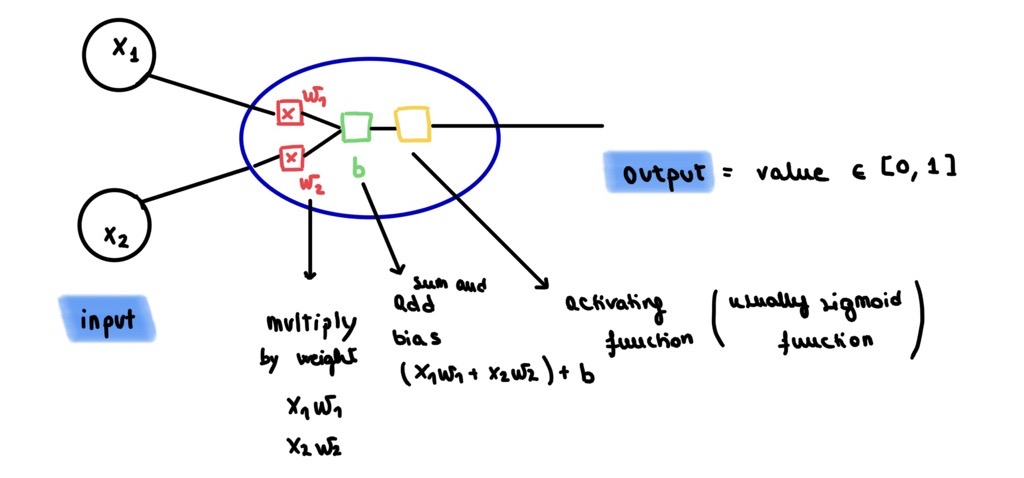
\includegraphics[width=0.75\columnwidth]{../figures_tex/neuron.png}
\caption{Two inputs ($x_1$ and $x_2$) neuron. Blue circle contains the operations performed in a neuron: \textcolor{red}{\textbf{multiply inputs to weights }} associated to the links, \textcolor{LimeGreen}{\textbf{sum inputs and add a bias $b$}}, \textcolor{Dandelion}{\textbf{apply an activating function}}. The outcome is a value belonging to $[0,1]$.}
    \label{fig:neuron}
\end{figure} 

\textit{Neural networks} are structures made of many neurons. These neurons are organized in layers, an example in \cref{fig:neural_ntw}. There are three types of layers: input layer, hidden layers and output layers. Input layers read the inputs, operations are performed in the hidden layer and output is generated in output layer. Hence, a neural network can be seen as a set of \textit{nodes} (the neurons) connected by \textit{edges} (the links with weights).
Given an input, each neuron in each layer performs computations and gives output that are inputs for the following neuron. This process of proceeding from the inputs to the outputs is called \textbf{feedforward}.
\begin{figure}[h]
    \centering
    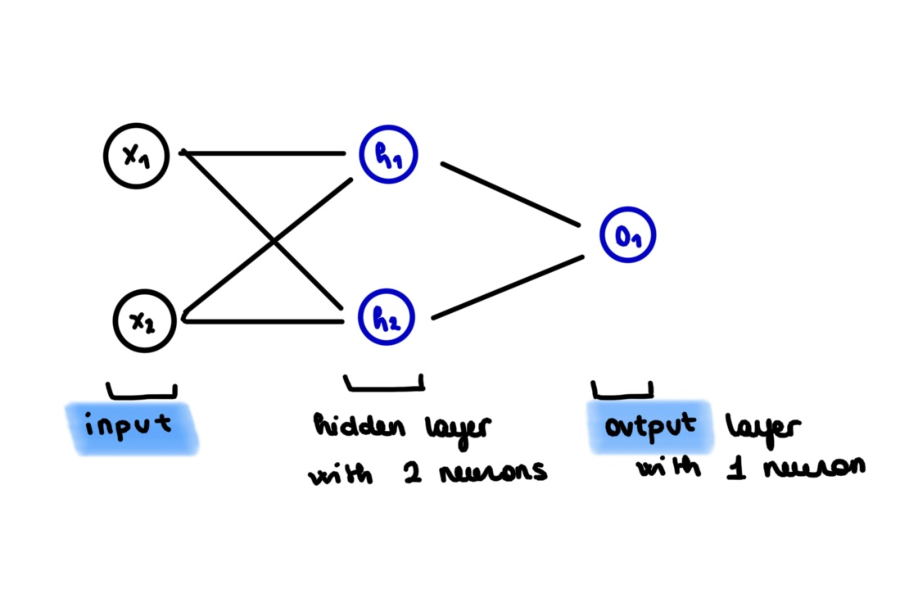
\includegraphics[width=0.6\columnwidth]{../figures_tex/neural_ntw.pdf}
    \caption{Example of a neural network: a structure made of neurons organized in layers.}
    \label{fig:neural_ntw}
\end{figure} 

A neural network needs \textit{training} in order to be able to perform a task. The standard way to train a network is by using a \textit{loss function}, which quantifies how good the output of the network is compared to the desired output. Often, the mean-squared error (MSE) is used
\[
\text{MSE} = \frac{1}{N} \sum_{i=1}^{N} (y_{\text{desired}} - y_{\text{predicted}})^2    
\]
where the sum is take over the training samples and $y$ indicates the value of the output in a specific neuron. From this simple formula we can already understand that a \important{smaller error implies a better prediction}. 

The training method proceeds in changing the weights in the network in the direction of the minimization of the loss function. It is therefore useful to denote as $L(\mathbf{w})$ the loss function as a function of the set of weights $\mathbf{w}$. In order to understand how the loss function changes when the weight are modified, we consider the derivative of the loss function with respect to the weights. Let us take for example the first weight $w_1$, the derivative $\partial L/\partial w_1$ is found by applying the chain rule
\[
\frac{\partial L}{\partial w_1} = \frac{\partial L}{\partial y_{\text{predicted}}} \frac{\partial y_{\text{predicted}}}{\partial w_1}    
\]
which is applied again to the second therm on the RHS following a path in the neural network which traces back to the location of the weight $w_1$. This procedure is called \textbf{backpropagation} since it accounts in propagating back the error in the network and identify the biggest sources of error. 

Once the derivative of the loss function is calculated, one needs to find a way of optimizing the network accordingly. A possible way of minimizing the loss function is by using \textbf{gradient descent} method. The weights are updated as follows:
\[
w \ \ \rightarrow w - \eta \frac{\partial L}{\partial w}    
\]
and the logic behind is that it changes the weight towards the direction of descent. In fact, a positive derivative means that a positive increase of the weight increases the loss function, from which a negative sign in front of the term. Vice versa for the negative sign. 

The training proceeds in steps and in each step the weights are optimized to decrease the error. There are many training samples in a dataset and a common training procedure randomly selects, at each step, one of the samples in the set and performs gradient descent. This procedure is called \textbf{stochastic gradient descent}.

\newpage

\subsection{CLSL framework}

We now consider a physical neural network (PNN). It is, again, a structure made of nodes and edges but, as opposed to ANN, they are not organized in layers and in principle there is no fixed pattern. However, just like an ANN, we divide the nodes in \textit{source nodes}, \textit{hidden nodes} and \textit{target nodes}. A generic PNN is shown in \cref{fig:general_graph}. These elements assume values of physical quantities and can be realized in real life. For example, in electric networks, the nodes assume values of potential and the edges of resistances.
\begin{figure}[h]
    \centering
    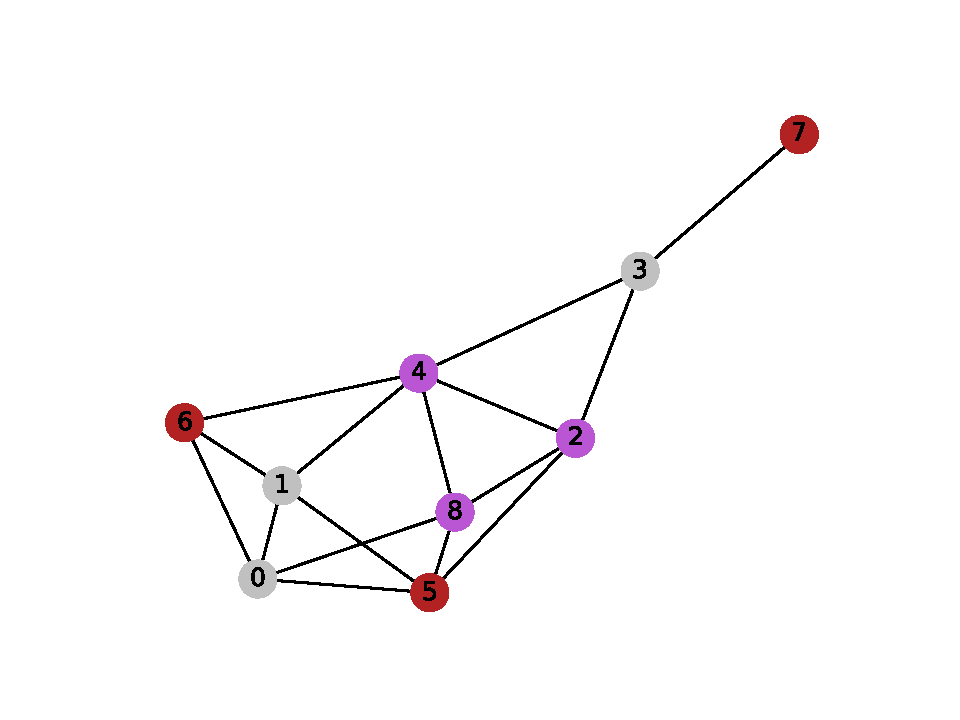
\includegraphics[width=0.6\columnwidth]{../figures_tex/general_graph.pdf}
    \caption{Example of a generic PNN. $5,6,7$ red dots denote input nodes, $0,1,3$ gray nodes denote hidden nodes and $2,4,8$ purple nodes denote target nodes.}
    \label{fig:general_graph}
\end{figure} 
The training goal here is to train the network to give desired outputs in the output nodes given certain inputs at the source nodes, just like in the ANN.

In a PNN, the values on the nodes follow from the minimization of an \textit{energy function}, as opposed to the feedforward procedure of ANN. For example, in electric networks, the function minimized is the power dissipated by the resistances. This, in turn, corresponds to satisfying Kichoff's law on current in the circuit of nodes and resistances, i.e. conservation of charge. In flow networks, minimization of power means conservation of flow.

\subsubsection{General formulation of the method}

Let us consdier a network with nodes indicized by $\mu$ and edges indicized by $j$. The \textit{physical degrees of freedom} (pof) belong to the set of variables $\{ x_{\mu}\}$. The \textit{learning degrees of freedom} (lof) belong to the set $w_j$ and play the roles of wieghts connecting the nodes. Given an initial condition $x_{\mu}(t=0)$ (part of the $x_{\mu}$ in the set given) and a set of weights, the physical degrees of freedom evolve to a steady state tha minimizes a \textit{physical cost function} $E(x_{\mu};w_j)$. Note that both $\{ x_{\mu} \}$ and $E$ depend on $\{ w_j\}$.

Inspired by \textit{contrastive Hebbian learning} (CHL), one considers two states of the network. The \textit{free state} $x_{\mu}^{F}$ in which the source nodes $x_S$ are constrained while the target $x_T^F$ and hidden $x_H^F$ equilibrate to the steady state. The \textit{clamped state} $x_{\mu}^{C}$ in which the source $x_S$ and the target $x_T^C$ nodes are constrained while only the hidden nodes $x_H^C$ equilibrate to the steady state. In the clampd state, the target nodes are nudged by an \textit{external supervisor} towards the desired $X_T$ values of outputs
\[
x_T^{C} = x_{T}^F + \eta \left[ X_T - x_{T}^{F} \right] 
\] 
with $\eta \ll 1$. In contrast with CHL, the nudge parameter is small, which fixes the problem of free and clamped state reaching two different local minima of the energy function.

The authors propose the following updating rule for the lof:
\[
\dot{\mathbf{w}} = \alpha \eta^{-1} \partial_{\mathbf{w}} \left\{ E(x_S, x_{H}^{F}, x_{T}^{F}) - E(x_S, x_{H}^{C}, x_{T}^{C}) \right\}   
\]

\begin{itemize}
    \item $\boldsymbol{\alpha}$ is a scalar \bf{learning rate}
    \item $\boldsymbol{\eta}$ is the \bf{nudging aplitude}.
\end{itemize}

% which corresponds to performing a gradient descent on the energy function with respect to the wiehgts. This means that the wieghts are updated towards a local minima of the energy function. 
The motivation behind this rule comes from the fact that we consdier a \important{physical} network, where generally one can partition the total energy $E$ as a sum over edegs $E = \sum_{j}E_{j}(x_{\mu}(j);w_j)$ of energies $E_j$ that only depend on the pof on the nodes that connect the edge $j$. Therefore, the learning rule is \important{local}. But does this rule effectively trains the network? The autors show (Appendix A in \cite{Stern}) that this updating scheme minimizes an \textit{effective cost function} that is not identical to the standard cost function but shares important features with it. They argue that minimizing the effective function mimics the minimization of a standard cost function. From how well the networks are trained, they observe that this affirmation is plausible. The CLSL approach shares many similarities with Equilibrium Propagation(EP) and the learning rule has the same form. However, in EP the learning rule minimizes an actual cost function.

Summarizing, the learning approach involves the minimization of an energy function and the implementation of the proposed updating rule. The former is motivated by physical plausability and the latter by inspiration from EP. %\textcolor{Orchid}{A comparison with minimization of an actual cost function is needed. They say EB is a type of contrastive learning.}

\section{Application to Electrical Netwroks}

The framework above can be applied in the context of electrical networks \cite{Dillavou}, in which nodes are connected by \textit{variable resistors}. When input voltages are applied at the source nodes $V_{S}$, the voltages at the output $V_{O}$ and hidden $V_{H}$ nodes are determined such that the total power dissipated by the resistances $\mathcal{P}$ is minimized
\[
\mathcal{P}  = \frac{1}{2} \sum_{j} \frac{\Delta V_j^2}{R_j}   
\]
where $j$ runs over the resistances $R_j$ and $\Delta V_j$ is the potential difference between the nodes that the resistance links.

We define the two types of states, as above. In the free state the source nodes $V^{F}_{S}$ are constrained, while $V^{F}_{H}$ and $V^{F}_{T}$ are determined by minimizing $\mathcal{P}$. In the clamped state, the source nodes $V^{F}_{C}$ are fixed to the source values, the target nodes are clamped 
\[
V^{C}_{T} = V^{F}_{C} + \eta \left( V^{D} - V^{F}_{C} \right)   
\] 
towards the desired output voltages $V^D$, while the hidden nodes are left to minimize $\mathcal{P}$. The parameter $0 < \eta \le 1$ quanitifies the importance of the nudge.

The final goal is to deliver the desired output $V^{D}$ to the target nodes. To do so, the network gets optimized by updating the values of the resistances following a certain \textit{learning rule}. The adaptation of the learning rule of CLSL in the context of electrical circuits would lead to the following \res{updating rule for resistances}
\begin{equation}
\boxed{\dot{R}_j = \frac{\alpha}{2\eta R_{j}^2} \left[ \left( \Delta V_{j}^{C}\right)^2 - \left( \Delta V_{j}^{F}\right)^2 \right] }
\label{eq:cont_rul_res}   
\end{equation}
where $R_{j}$ is the selected resistance to update, $\Delta V_{j}^{C}$ is the potential difference between the nodes that it connects in the clamped state and $\Delta V_{j}^{F}$ the difference in the free state. In the paper \cite{Dillavou} they define
\[
\gamma = \frac{\alpha}{2\eta}
\]
as the learning rate.

In the experiment, they have discrete resistors and the rule above gets approximated with the following 
\begin{equation}
\boxedapp{\dot{R}_j = \begin{cases} 
    +\delta R & \text{if} \ |\Delta V^{C}_{j}|>|\Delta V^{F}_{j}| \\
    -\delta R & \text{otherwise}
 \end{cases}}
\label{eq:disc_rul_res}
\end{equation}
which consists in taking the sign of \cref{eq:cont_rul_res} and multipy it by the value $\delta R$.

We can also reformulate the theory in terms of conductances $g_j = 1/R_j$, the updating rule of wihch can be derived from the power dissipated
\[
\mathcal{P}  = \frac{1}{2} \sum_{j} \frac{\Delta V_j^2}{R_j} = \frac{1}{2} \sum_{j} g_j \Delta V_j^2.
\]
In terms of the learning rate $\gamma$, the \cond{updating rule for conductances} reads
\begin{equation}
    \boxedc{\dot{g}_j = \gamma \left[ \left( \Delta V_{j}^{F}\right)^2 - \left( \Delta V_{j}^{C}\right)^2 \right] }   
\label{eq:cond_update_cont}
\end{equation}

\subsection{Simple Start: Voltage Divider}

One of the simplest networks we can consider is a voltage divider, shown in \cref{fig:voltage_divider_graph}. 
\begin{figure}[h]
    \centering
    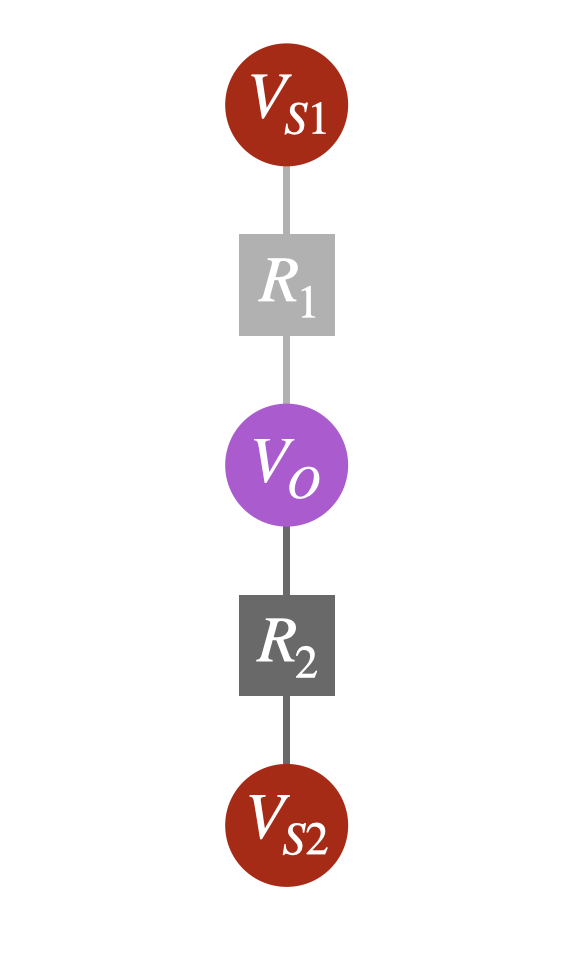
\includegraphics[width=0.2\columnwidth]{../figures_tex/voltage_divider_graph.png}
    \caption{Schematic representation of the voltage divider considered in this section. It has two input nodes (red dots) with voltages $V_{S1}$ and $V_{S2}$, one output node with voltage $V_O$ and two edges with resistances $R_1$ and $R_2$.}
    \label{fig:voltage_divider_graph}
\end{figure} 
It has three nodes, two of type source and one of type output with potential, respectively, $V_{S1}$, $V_{O}$ and $V_{S2}$. These three nodes are connected by two resistances, $R_1$ and $R_2$, as in figure. The goal in training this network is to deliver a desired voltage of $V_{D} = 4V$ on the output node with voltage $V_O$, when imposing voltages of $V_{S1}=5V$ and $V_{S2}=0V$. At the beginning, the resistances are initiated to a value of $R = 50 k \Omega$. In this first section, we are trying to reproduce the results shown in the paper \cite{Dillavou}, we are thus adopting the same setting and choice of parameters.

In the free state, only the source voltages are imposed while the value of the output voltage $V_O$ minimizes the total power dissipated by the two resistances in the system,
\[
\mathcal{P} = \frac{\Delta V_1^2}{R_1} + \frac{\Delta V_2^2}{R_2}
\] 
where $\Delta V_1 = V_{S1} - V_{O}$ and $\Delta V_2 = V_{O} - V_{S2}$. For this simple system, it is possible to explicitly solve $\partial \mathcal{P}/\partial V_O = 0$ finding the relation
\[
R_2 (V_1 - V_O) = R_1 (V_O - V_2)
\]
which suggests that the ratio between the resistances in the steady state is 
\begin{equation}
\frac{R_1}{R_2} = \frac{V_1 - V_O}{V_O - V_2}.
\label{eq:res_ratio_simple}
\end{equation}
In the case of the parameters we choose at the beginning of this section, we can state that when the network reaches the desired configuration, the ratio between the resistances should be $R_1/R_2 = 5/4 = 1.25$.

The training consists in steps, each of which results in an update of the edges in the network following the updating rule chosen. To reproduce the results in the paper \cite{Dillavou}, we first select the updating rule \cref{eq:disc_rul_res}. This rule is discrete, it can update with a value of either $+\delta R$ or $-\delta R$, as opposed to a continuous rule, which updates with a value that in principle can be any real number. Before looking at the results of the training process on this system, we introduce the mean-squared error (MSE)
\[
C = \sum_{i \in \text{output nodes}} (V_{i} - V_{D,i})^2,
\]
this is a parameter that quantifies how far the output voltages $V_i$ are from their desired values. Thus, the goal in the training is to reduce the MSE as much as possible.

We show the results of the training in \cref{fig:voltage_div_1} and we want to compare them with the first $100$ training steps shown in Fig. 2(c) of the paper \cite{Dillvaou}. 
\begin{figure}[h]
    \centering
    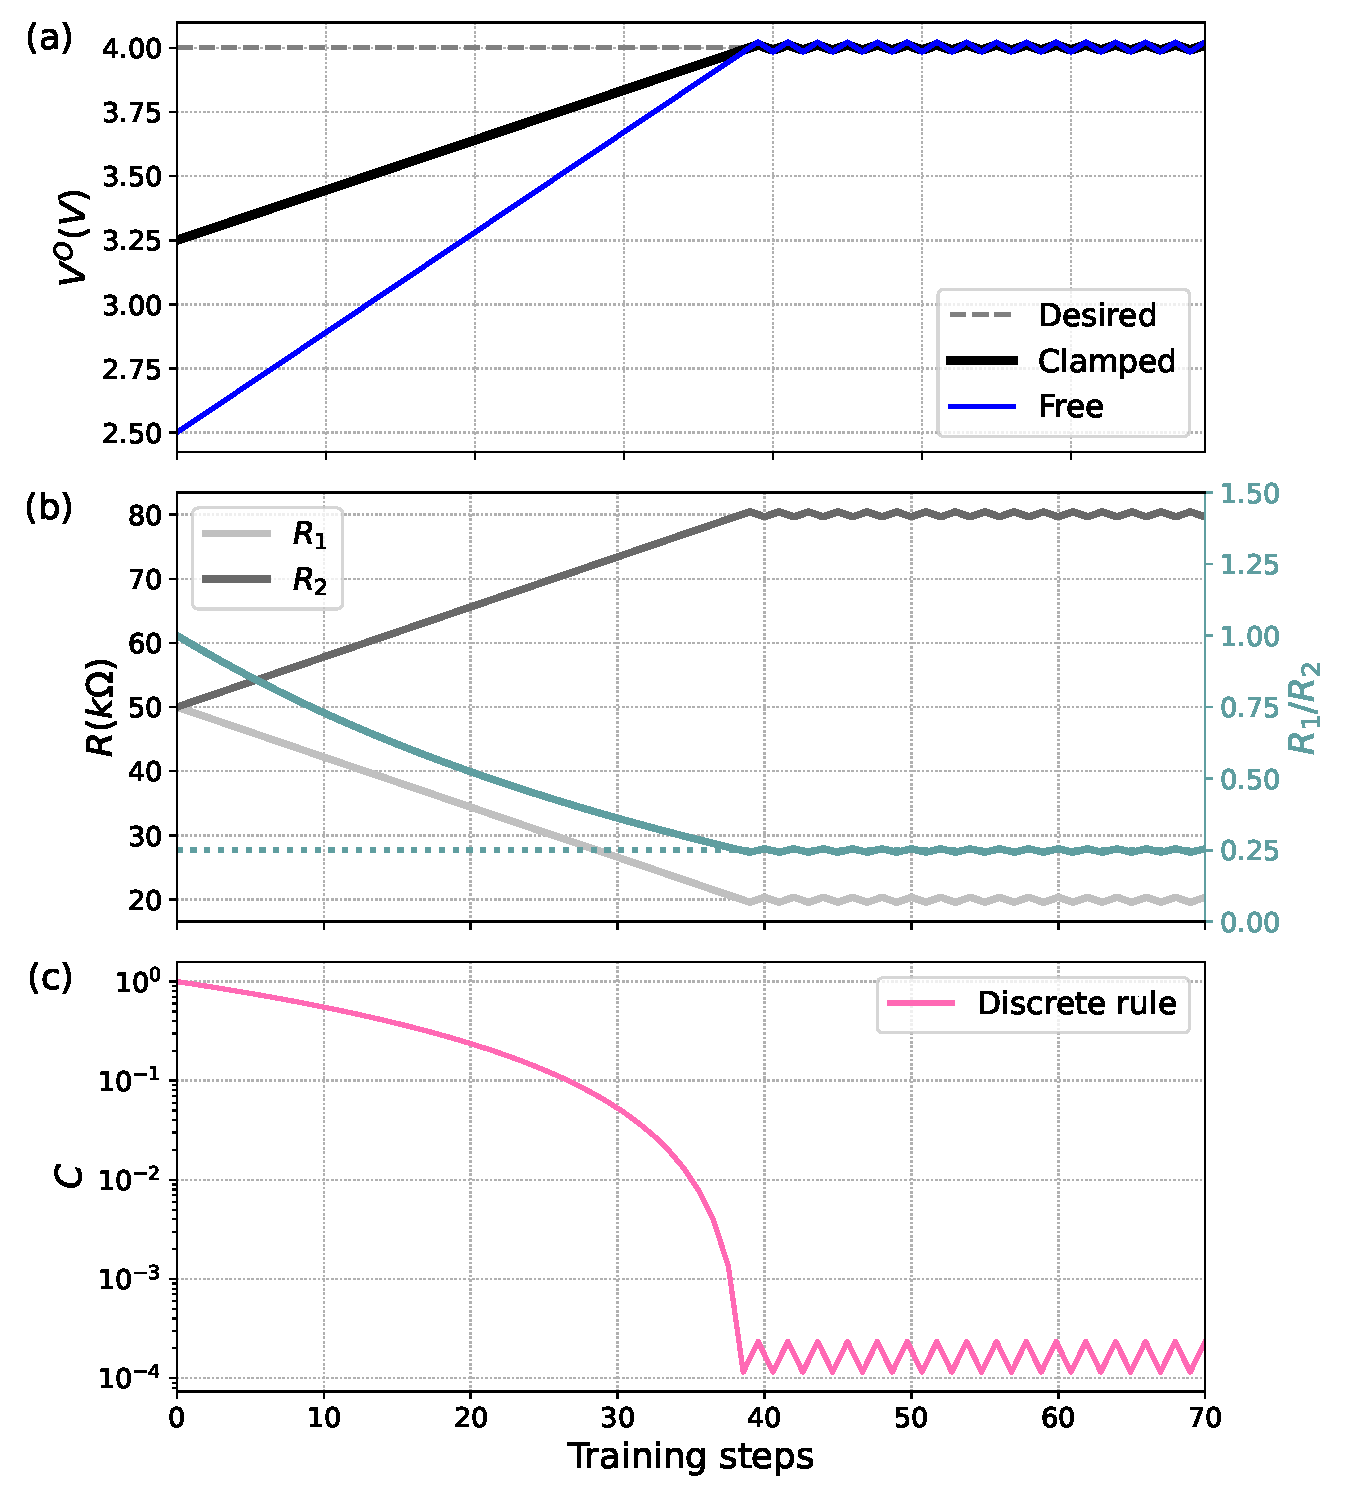
\includegraphics[width=0.5\columnwidth]{../figures_tex/volt_res_mse_simp.pdf}
    \caption{Training of the voltage divider in \cref{fig:voltage_divider_graph} with $V_{S1}=5V$, $V_{S2}=0V$, $V_{D}=4V$ and discrete rule of \cref{eq:disc_rul_res}. The clamping rate is set to $\eta=0.5$. In (a) the plot of the voltage measured in the output node, $V_O$, during training, in the free state, clamped state. The dashed line indicates the desired voltage $V_D$. (b) Shows the values of the resistances in the edges $R_1$ and $R_2$ during training. The green line represents the ratio $R_1/R_2$, while the dashed green line the desired ration that follows from \cref{eq:res_ratio_simple}. In (c) the plot of the MSE.}
    \label{fig:voltage_div_1}
\end{figure} 
We observe that the training reduces the MSE of four orders of magnitude in $40$ steps, with a behaviour fairly similar to the results in the paper. It is after this value that we can notice the limitation of this discrete rule: the system is not adaptive. In fact, as the network gets trained and difference between the potentials in the free and clamped state
\[
|\Delta V^{C}_{j}|-|\Delta V^{F}_{j}| = \sigma
\]
becomes smaller, the resistances still get a big contribution to their change in value. In our case, the system gets stuck and oscillates between two configurations, spoiling the training procedure thereafter. Experimentally, the presence of noise enables to get out of these problematic configurations and explore the solution space. Recall that, in this simple case, there is an infinite set of solutions for the values of the two resistances: they only need to satisfy \cref{eq:res_ratio_simple} to be solutions. However, as shown in Fig. 3(a) in the paper, the presence of noise only allows the selection of a few favourable, randomly picked configurations in which the MSE decreases of a few orders of magnitude, but there is no overall improvement in the training process.

Therefore, we decide to compare the discrete rule of \cref{eq:disc_rul_res} with the continuous rule of \cref{eq:cont_rul_res}, the result is shown in \cref{fig:volt_res_mse_simp_cont}. 

\begin{figure}
\begin{subfigure}{.5\textwidth}
  \centering
  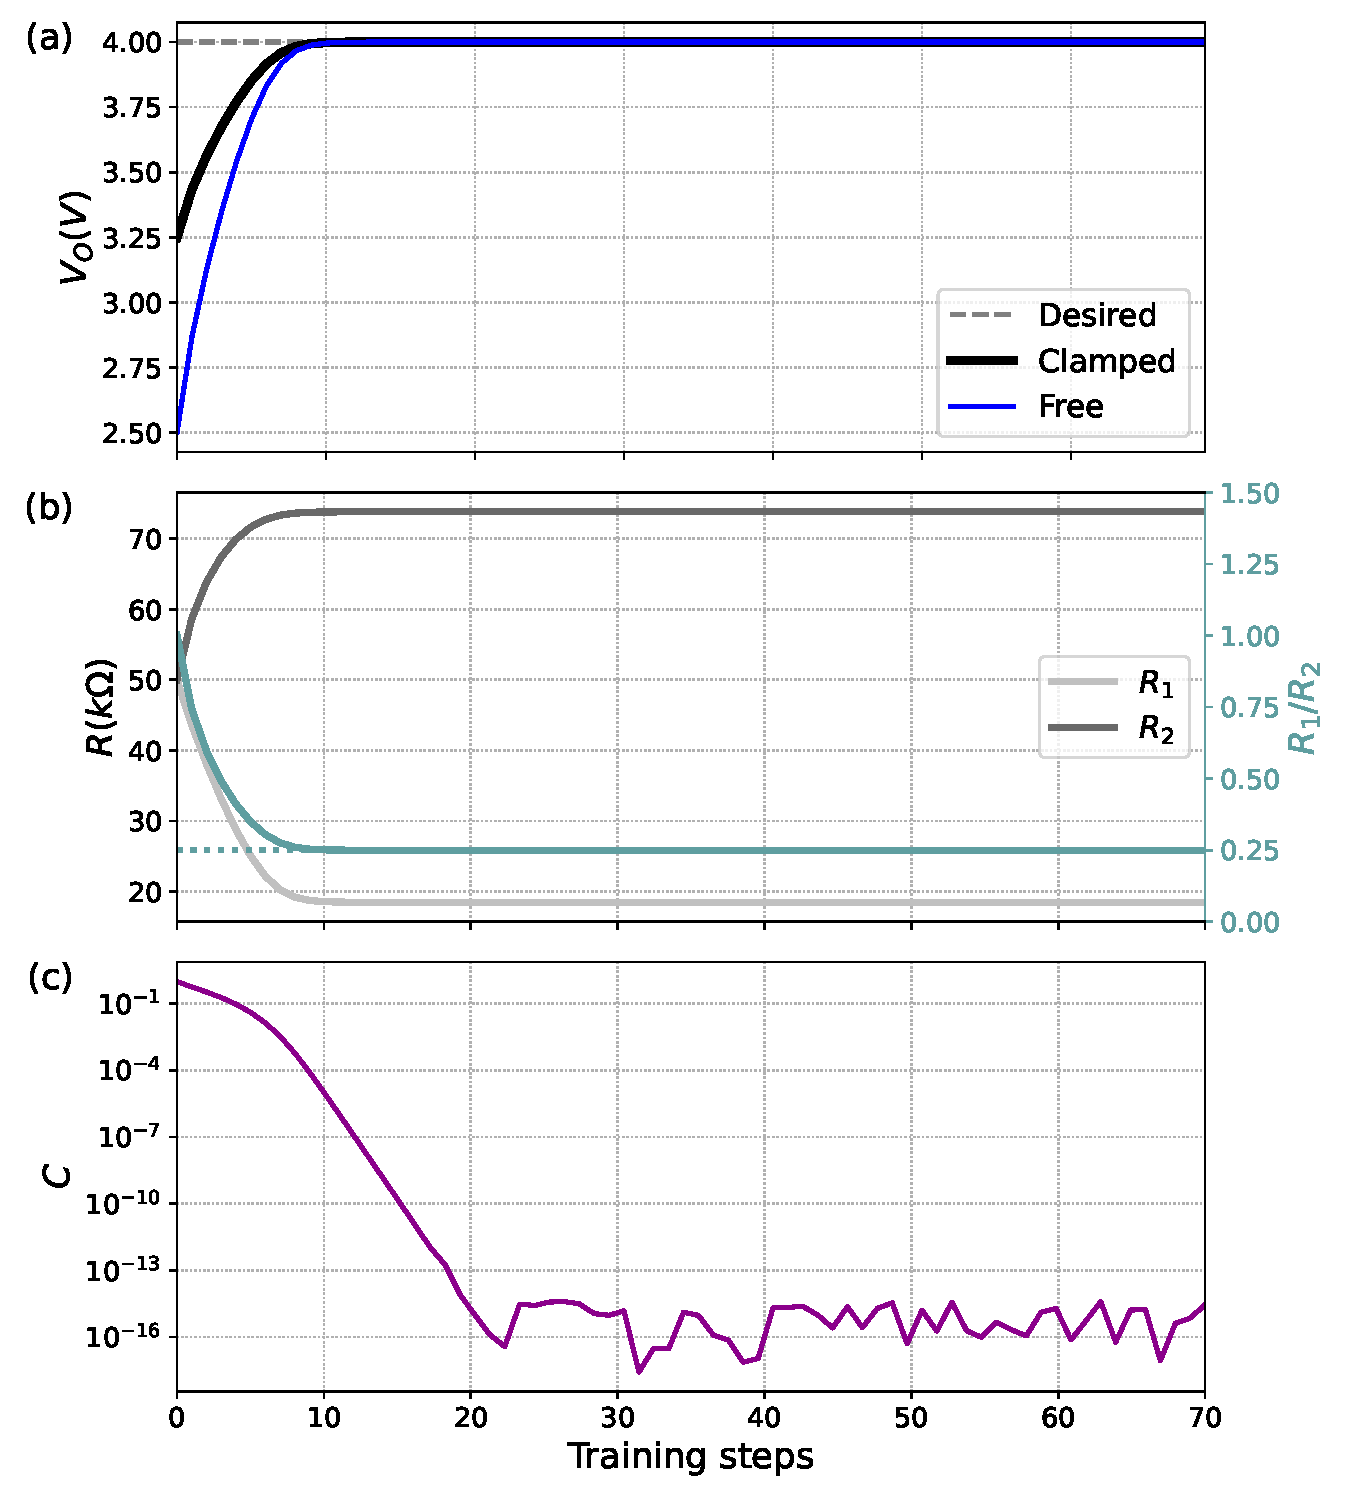
\includegraphics[width=0.9\columnwidth]{../figures_tex/volt_res_mse_simp_cont.pdf}
\end{subfigure}%
\begin{subfigure}{.5\textwidth}
  \centering
  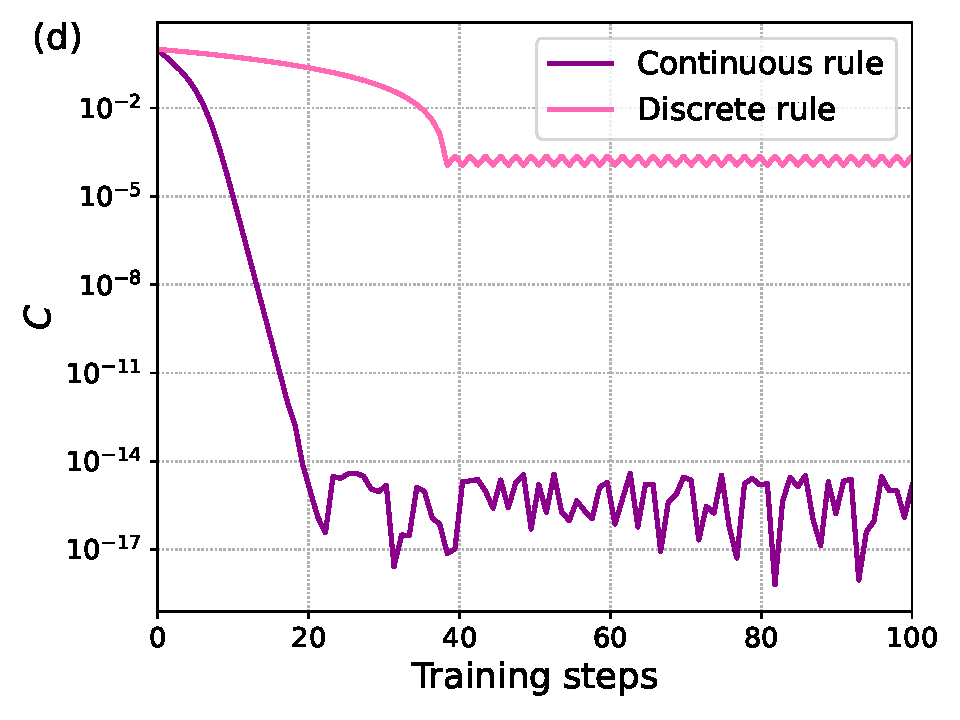
\includegraphics[width=0.8\columnwidth]{../figures_tex/res_disccont_simple.pdf}
\end{subfigure}
\caption{(a), (b), (c) Training the voltage divider with continuous rule on resistances. The nudging parameter $\eta=0.5$ and $\alpha=5\times 10^3$. (d) Plot of the MSE resulting from implementing the discrete rule in \cref{eq:disc_rul_res} and the continuous rule in \cref{eq:cont_rul_res} on the resistances of the voltage divider.}
\label{fig:fig}
\end{figure}


We can now compare the discrete and continuous rule by plotting the MSE that results from both training methods, this is shown in \cref{fig:res_disccont_simple}. We can see how the implementation of the continuous rule enables to reach configurations with a MSE many orders of magnitude smaller than what obtained implementing the discrete rule. There are some oscillations of the MSE in the continuous rule after it has reached a value of the same order of magnitude as the one possessed by the machine precision.

From the results obtained in this simple system, we decided to pursue the idea of finding a physical system that enables the experimental realization of the continuous version if the updating rule on resistances. In our fist attempt, we will consider ionic channels with memristive properties. But, before introducing such systems, in the next section we perform the same analysis in a more complex network.


\newpage
\subsection{More General: $3$-input $3$-output Network}

Let us consider a network made of $9$ nodes connected by $16$ resistances. Of these nodes, $3$ are source nodes, $3$ target nodes and $3$ hidden nodes. A similar three-input three-output network was considered for allostery tasks in \cite{Dillavou}.
\begin{figure}[h]
    \centering
    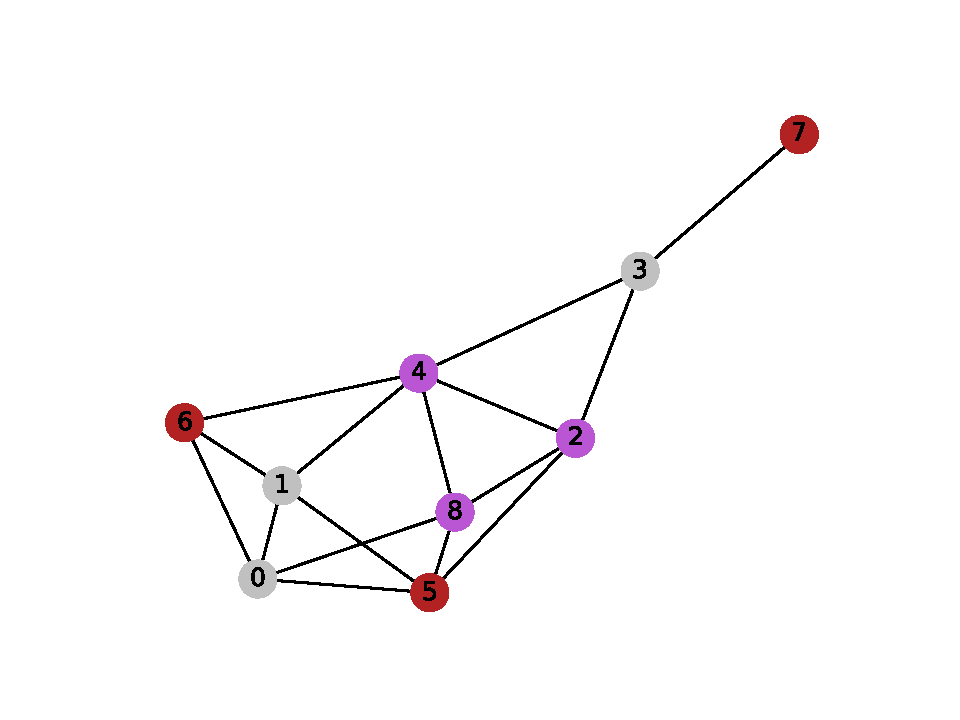
\includegraphics[width=0.5\columnwidth]{../figures_tex/general_graph.pdf}
    \caption{A three-input (red nodes), three-output (purple nodes) network with $16$ edges. The allostery task consists in delivering $3V$ in the output nodes, giving $0$, $1$ and $5V$ to the source nodes. The resistances are initiated to a value of $50k\Omega$.}
    \label{fig:res_disccont_simple}
\end{figure}

We first implement the discrete version of the updating rule for resistances and obtain the result shown in \cref{fig:general_training_discrete}. As also discussed in previous work (see \cite{Stern} Appendix D), learning degrees of freedom in physical systems (in the case here considered, the resistances) share a physical limitation, i.e. their value can not be negative. Therefore, the capacity of the networks considered to learn mappings between sources and targets is limited. Different approaches to circumvent this issue have been explored (works cited in \cite{Stern}, still to be explored), but the authors of the papers we are following simply cut off the values of resistances. In the discrete case, the resistances can assume values between $781\Omega$ and $100k\Omega$.
\begin{figure}[h]
    \centering
    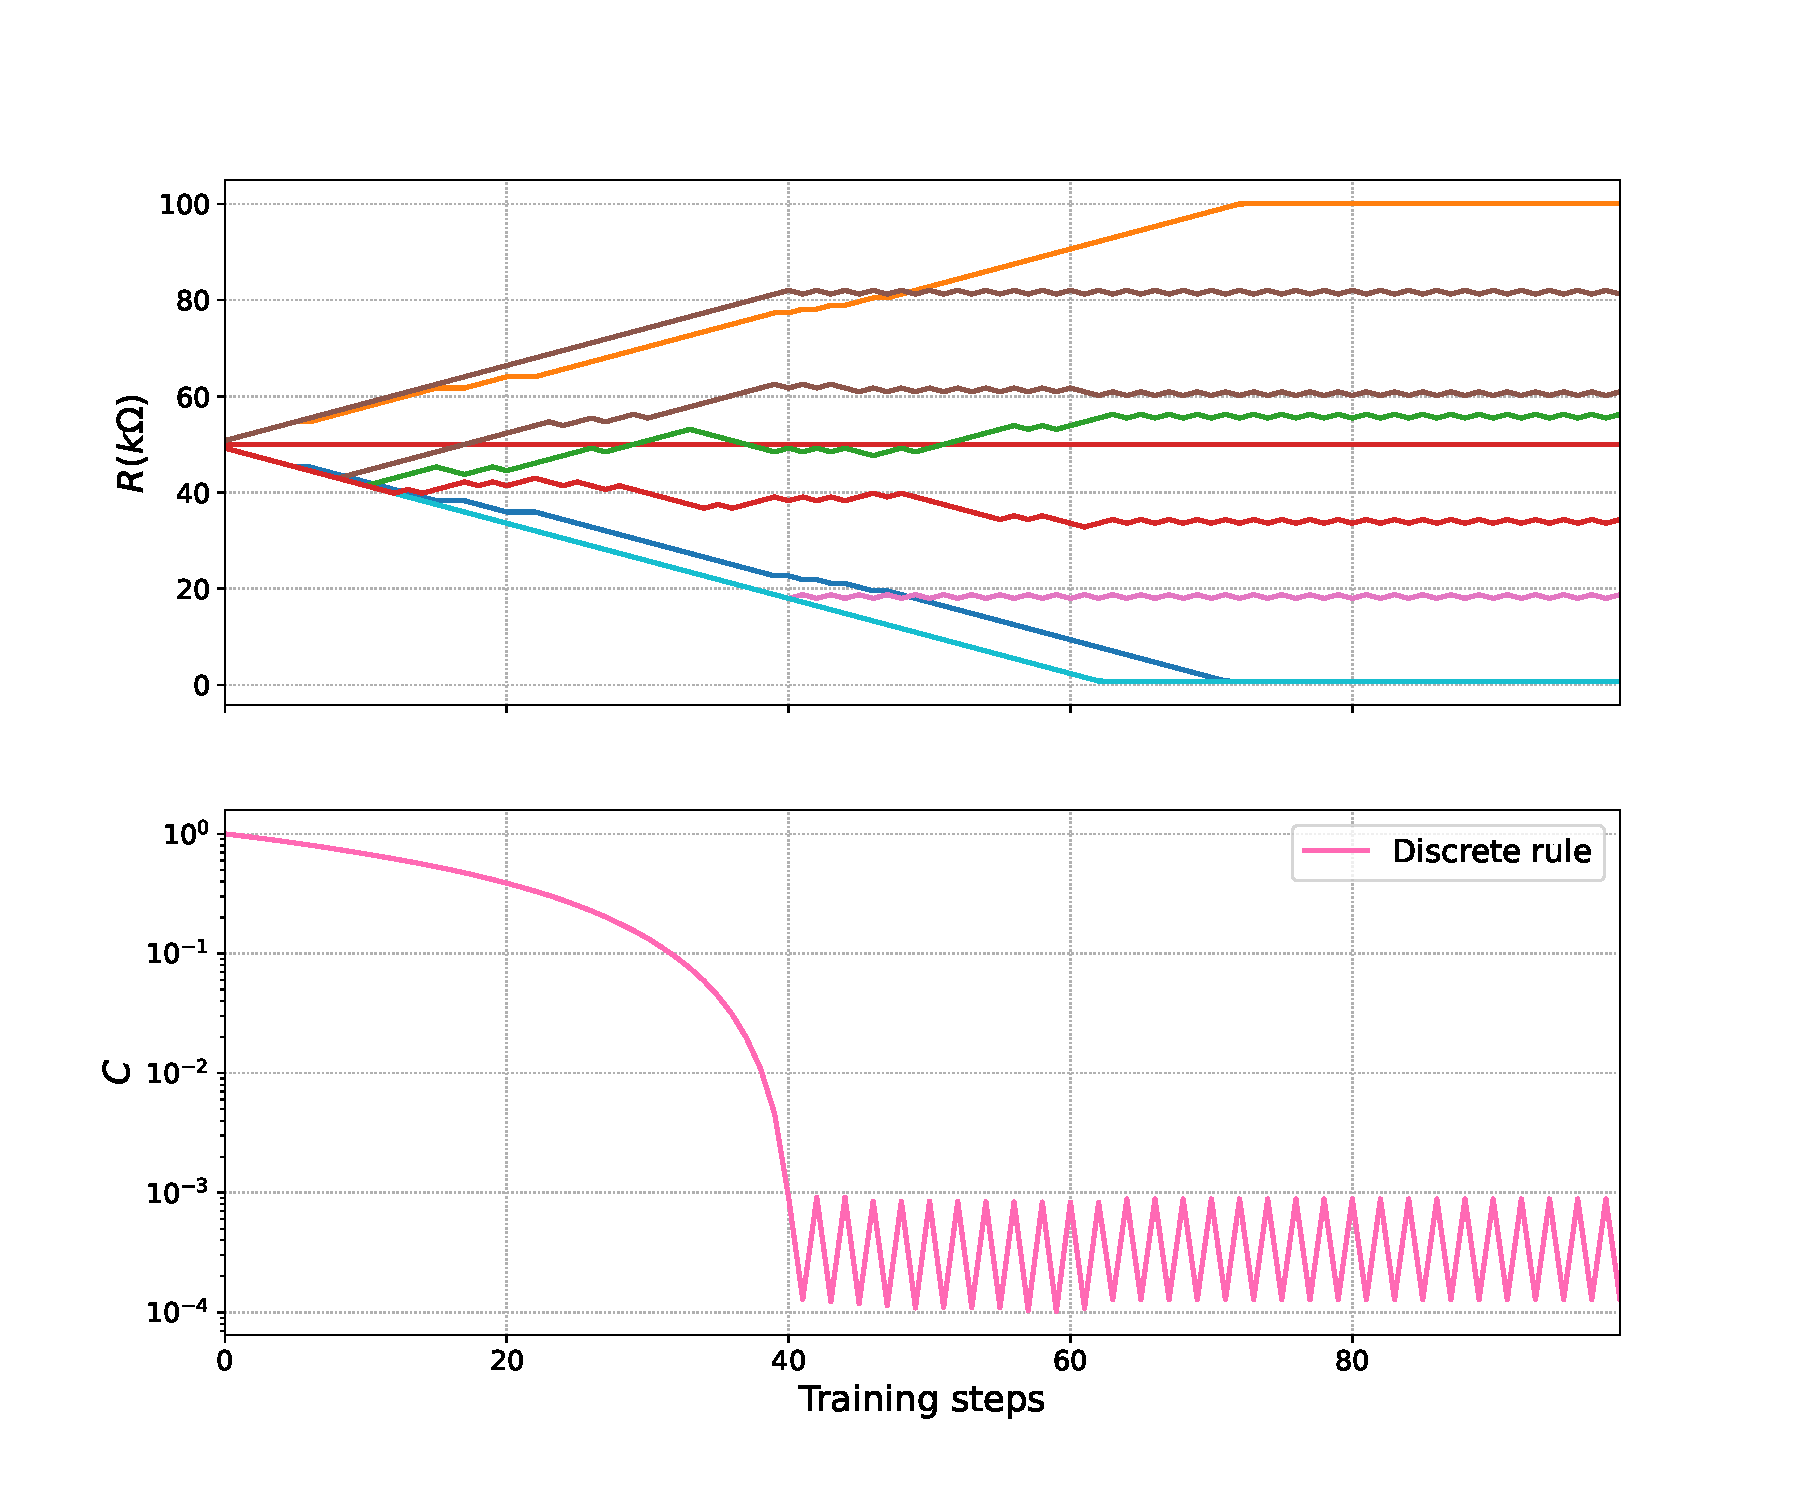
\includegraphics[width=0.5\columnwidth]{../figures_tex/general_training_discrete.pdf}
    \caption{Training the three-input three-output network with the discrete rule for resistances with $\eta = 0.5$.}
    \label{fig:general_training_discrete}
\end{figure}

Comparing the behaviour of the MSE with the one obtained from the implementation of a similar network (see Fig. 3(a) in \cite{Dillavou}), we find that our training reaches the same order of magnitude as theirs. Recall that we do not implement noise, this forbids getting stuck between two configurations as, on the other hand, happens in our model.

Regarding the choice of the value of the nudging parameter $\eta$, from the theory \cite{Stern} we know that when $\eta \ll 1$, the coupled learning rule mimics the optimization of an effective cost function. On the other hand, the choice of $\eta \sim 1$, as suggested by contrastive Hebbian learning, can affect negatively physical learning, especially in nonlinear networks where the energy landscape in nonconvex and could cause the free and clamped state to reach two different minima, spoiling the training. Therefore, the theory suggests small values of nudging parameter $\eta$. However, it was shown \cite{Stern} that
\[
\left[ \Delta V^C \right]^2 - \left[ \Delta V^F \right]^2 \sim \eta^2
\]
which suggests that in an experimental setting when the system is approaching a solution, noise dominates if $\eta$ is too small. Therefore, the conclusion is that the nudge parameter should be small so that the optimization process gives a good estimate of the desired gradients, but not too small otherwise the learning is dominated by the noise. So far, we have used $\eta = 0.5$ with the sole purpose of replicating the results in the paper and validate our code. 

From these results, we can conclude that both the physical limitation on the values of resistances and the discreteness of the updates, still too big when the system approaches a solution, limit the accuracy of the training.

We now switch to the implementation of the continuous rule on the same network. With a fixed value for the nudge parameter $\eta=0.5$, we still have the freedom to chose the value for the learning parameter $\alpha$. However, changing the latter only changes of an overall factor the learning rule: the behaviour of the training in time does not change but only the speed is affected. In order to obtain the same time-interval for the training, we set a value of $\alpha = 5 \times 10^3$. The result is shown in \cref{fig:general_training_continuous}.
\begin{figure}[t]
    \centering
    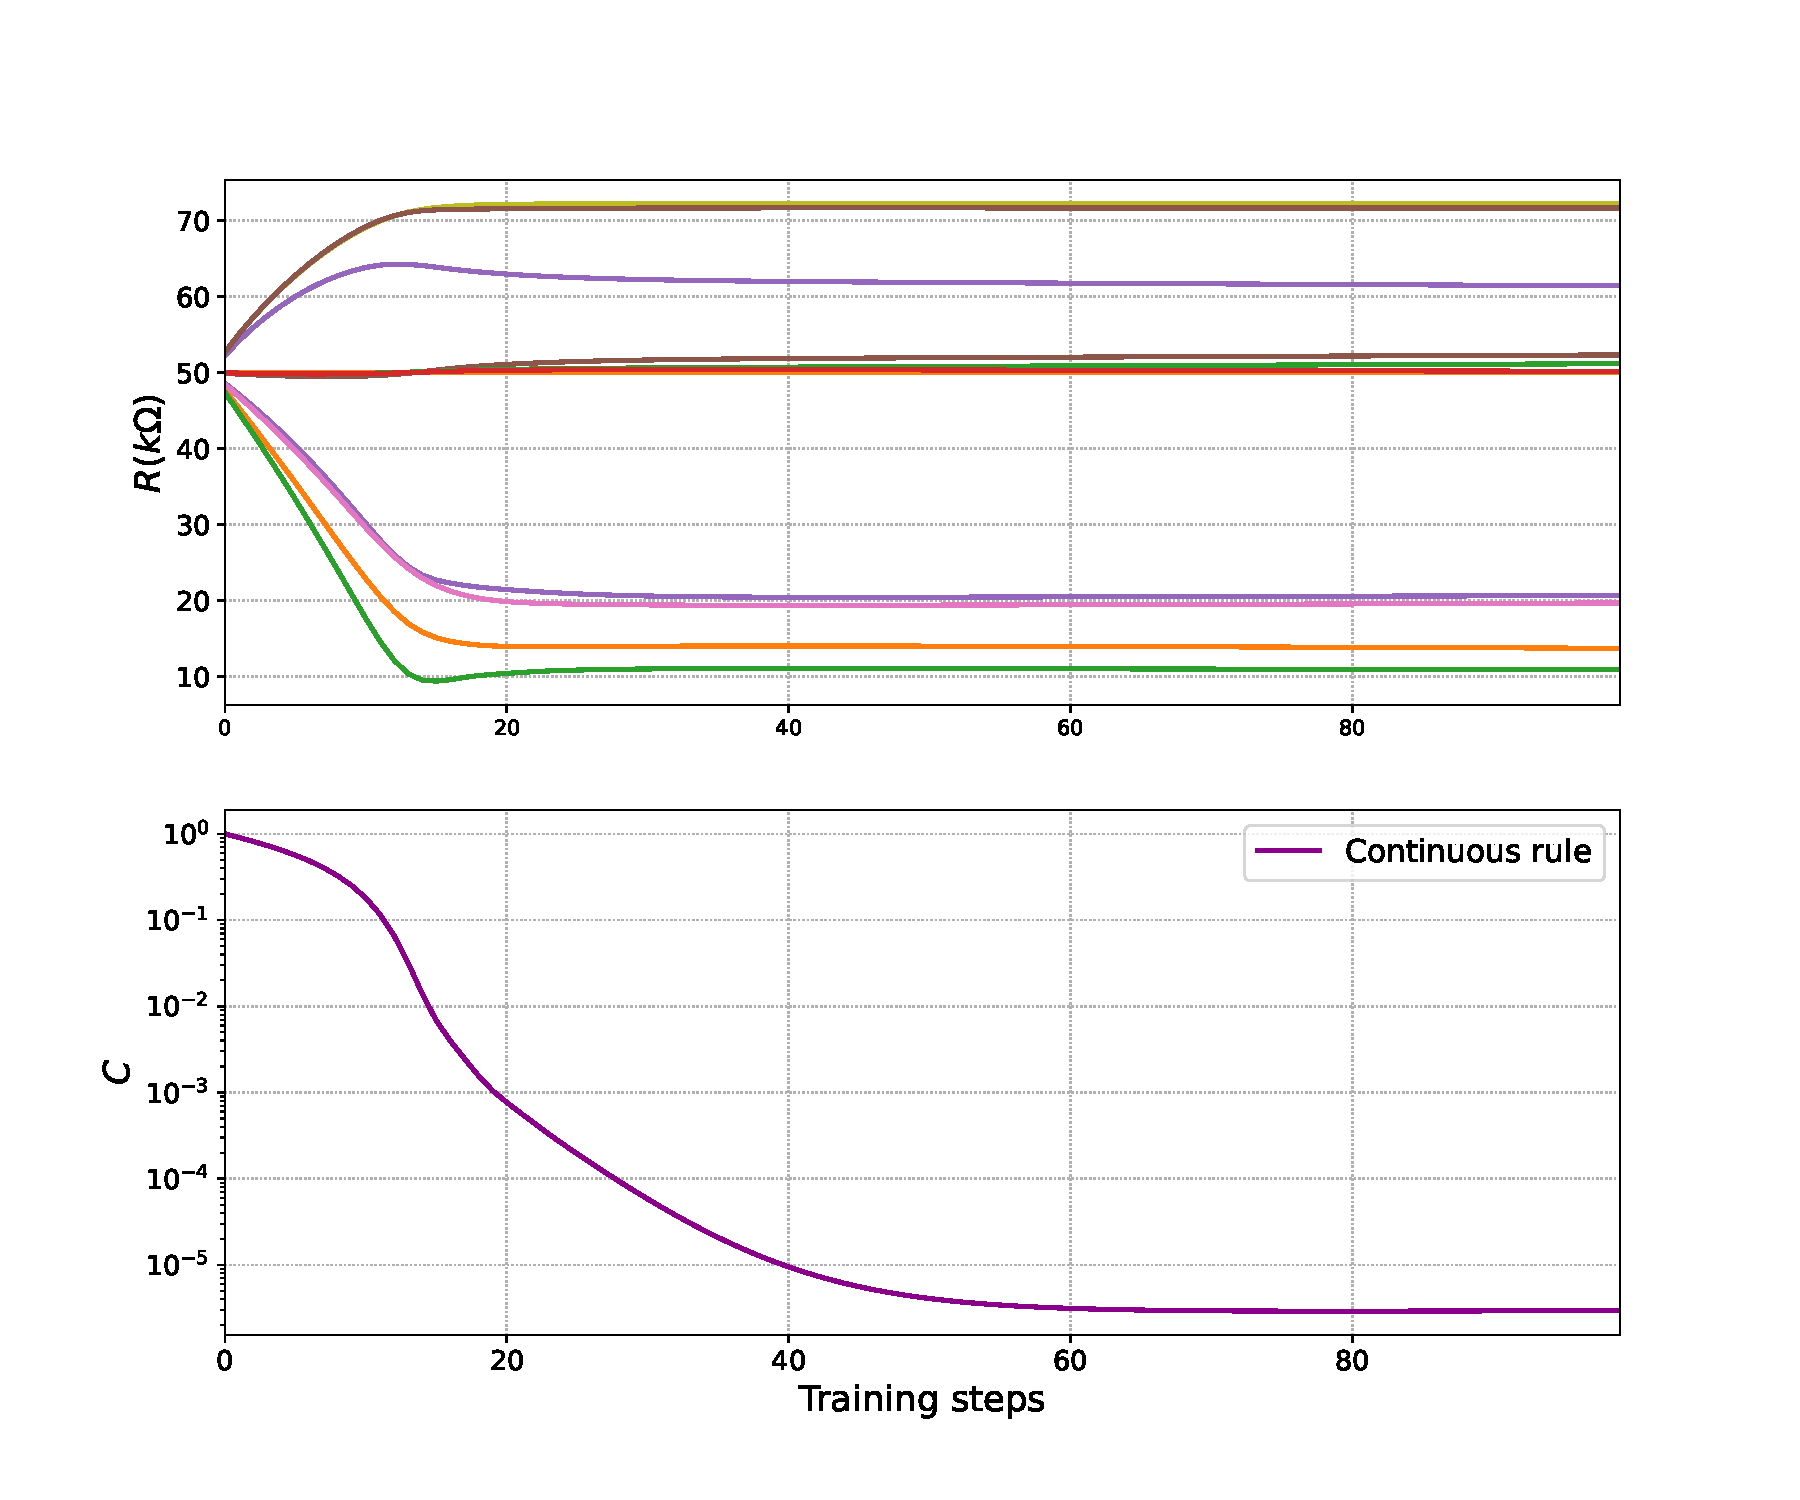
\includegraphics[width=0.5\columnwidth]{../figures_tex/general_training_continuous.pdf}
    \caption{Training the three-input three-output network with the continuous rule for resistances. Here $\eta = 0.5$ and $\alpha = 5 \times 10^3$.}
    \label{fig:general_training_continuous}
\end{figure}

A comparison between the two rules is now possible, it is shown in \cref{fig:general_training_comparison}.
\begin{figure}[t]
    \centering
    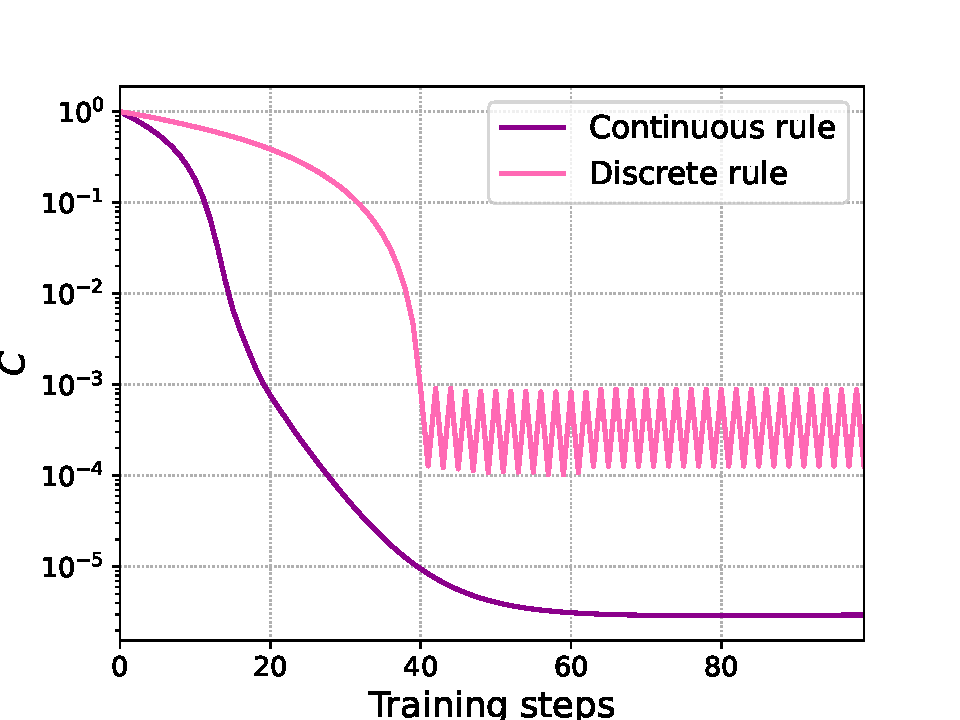
\includegraphics[width=0.5\columnwidth]{../figures_tex/comparison_general.pdf}
    \caption{MSE resulting from training a network with a discrete and continuous rule. Here $\eta = 0.5$ and $\alpha = 5 \times 10^3$.}
    \label{fig:general_training_comparison}
\end{figure}
The implementation of the continuous rule results in a better precision of the desired outputs. 

However, I am still trying to understand why the the error seems to plateau between $10^{-5}$ and $10^{-6}$ instead of keep decreasing. To investigate his point further, I run the algorithm in the continuous setting for more time steps, the result is shown in \cref{fig:continuous_long}. We can see that the optimization proceeds and, even if not in a monotonic way, the error decreases of many orders of magnitude.
\begin{figure}[h]
    \centering
    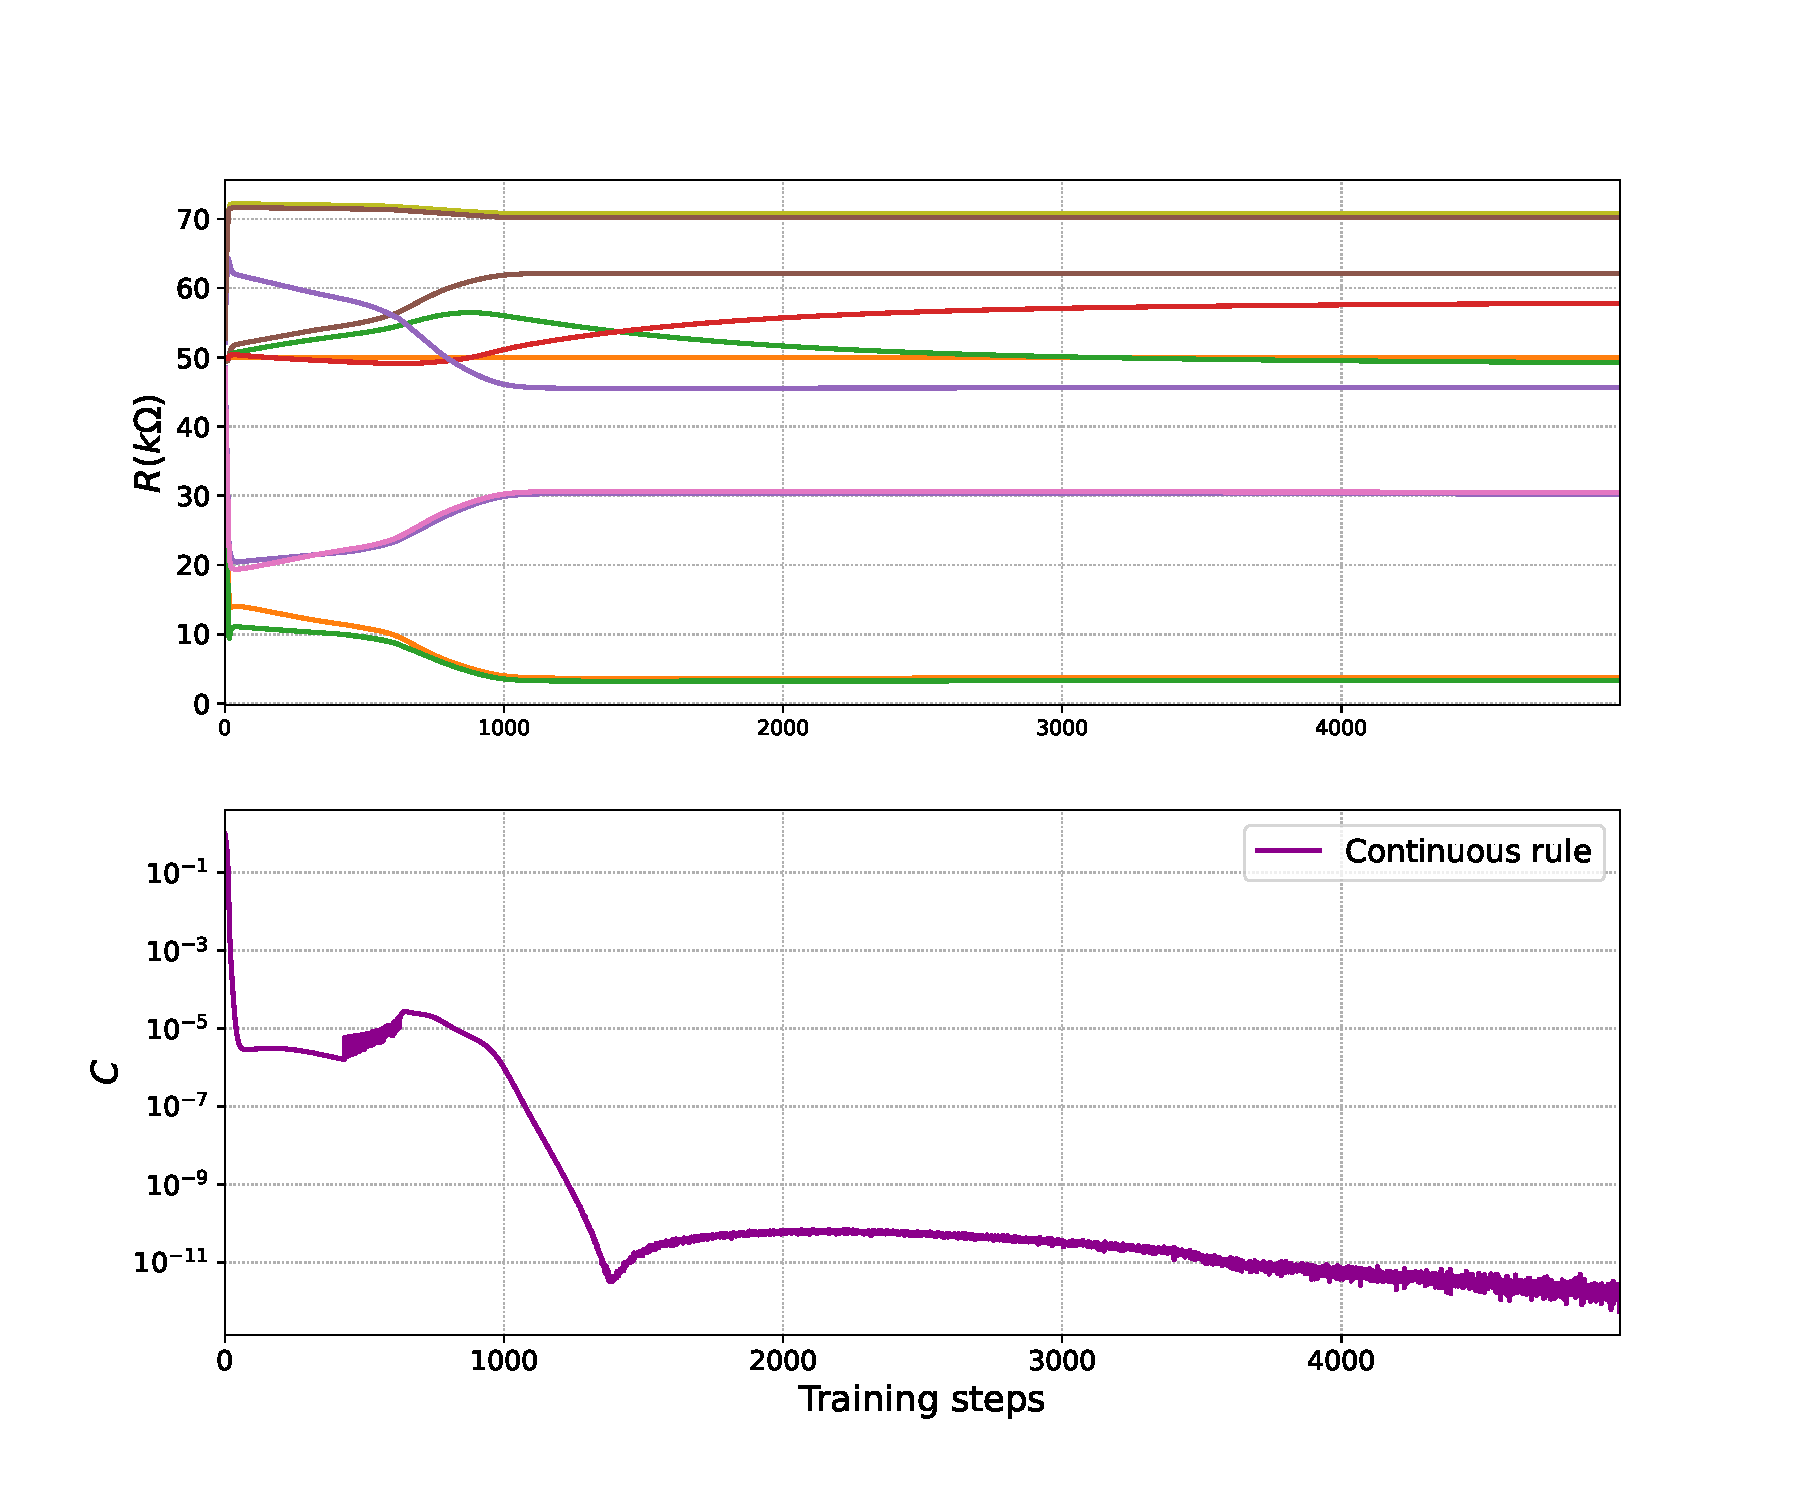
\includegraphics[width=0.5\columnwidth]{../figures_tex/continuous_long.pdf}
    \caption{MSE resulting from training a network with a continuous rule for a long period of time. Here $\eta = 0.5$ and $\alpha = 5 \times 10^3$.}
    \label{fig:continuous_long}
\end{figure}
Since the theory suggests a small value of nudging parameter $\eta$, we compare the training of the continuous rule for different values of this parameter, the result is shown in \cref{fig:general_etas}. 
\begin{figure}[h]
    \centering
    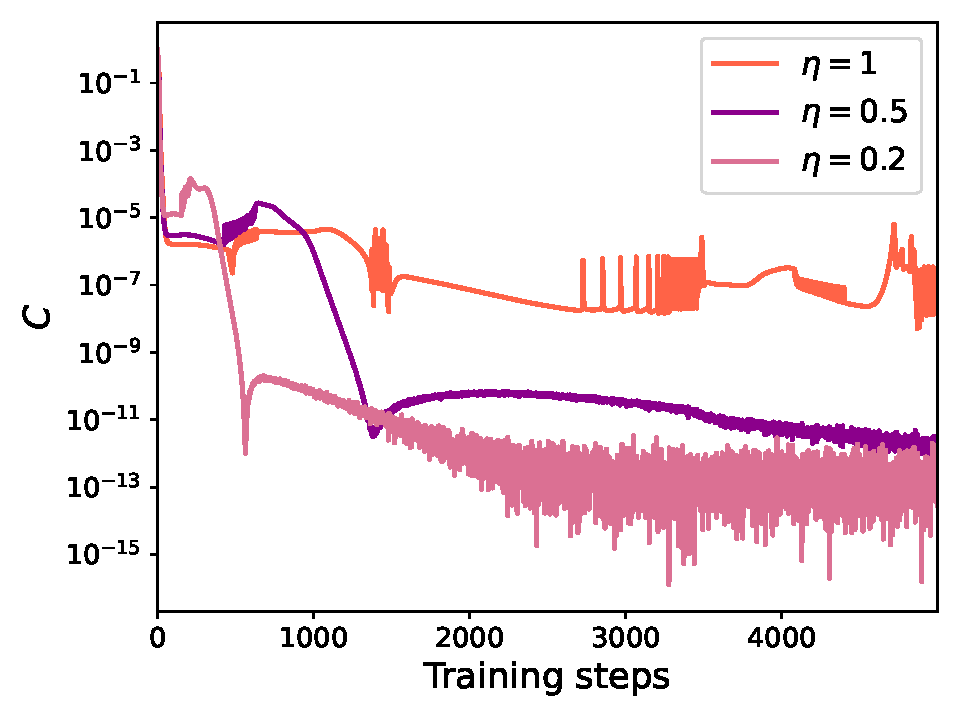
\includegraphics[width=0.5\columnwidth]{../figures_tex/general_etas.pdf}
    \caption{MSE resulting from training a network with a continuous rule for three different values of nudging parameter. Here $\alpha = 5 \times 10^3$.}
    \label{fig:general_etas}
\end{figure}
We indeed see that a smaller nudging parameter makes training faster and more accurate on the long run.
%Say that continuous is better, make graph. Don't know why it does not continue to improve of more orders of magnitude. I even observed that it gets worse as the time increases more, show other graph. Changing the nudging parameters for values of 0.5 below only speeds up the training, without improving it, as also observed in \cite{Stern} see Appendix A.

As a last note, I experimented that the geometry of the network really influences the training. Due to the physical limitation on the values of resistances, many geometries lead to a situation in which, after some of the resistances reach the cut-off, the training is slowed down considerably. 

For further developments, it will be necessary to consider methods that avoid going to negative values of the physical quantities of edges. Moreover, it would be interesting to understand better the role of the geometry on the training. To do this, we should first introduce a metric in the network and then study the behaviour of the training as a function if relative distance between inputs-outputs and as a function of the connectivity. But these two parameters are just an example, we can think of more.

\clearpage
\section{Conical Microfluidic Memristors}

The goal of this work is to physically realize a trainable network. We discussed in the last section the limitation of variable resistors, not continuously adjustable, on the accuracy of the output voltages. Moreover, the system needs a supervisor that reads the voltages on output nodes and clamps them depending on the sign of the difference between the voltages in the free and clamped configurations.

On the direction towards a more precise and efficient physical system, we consider resistors that can change their value continuously. Moreover, we would like them to be autonomous, meaning that they don't need the advice of a supervisor. Our first attempt is to substitute resistors with memristors. These devices can change the value of their resistance continuously and have memory, in the sense that the value of the resistance depends on the history of the applied voltage. Perhaps, this property of memory could make the system autonomous.

There are many physically realized memrisotrs, we choose to work with conical channels filled with an aqueous electrolyte since they offer a wide range of achievable values of resistances, they are fast, cheap and easy to fabricate. In previous works \cite{cone1, cone2}, these devises were used to perform neuromorphic computing, a computational paradigm that seeks inspiration from the way the brain processes information. They successfully reproduced some neural behaviours, like neural spiking, all-or-none action potentials and short-term plasticity, just to mention some.

\subsection{The model}

Let us consider a single conical channel, shown in \cref{fig:conical_channel}, of length $L = 10\mu$m. It has a base radius of $R_{b} = 50$nm (radius at $x=0$), a tip radius (at $x=L$) of $R_t = 50$nm and the radius in between is given by $R(x)=R_b-x\Delta R/L$. The channel connects two reservoirs of electrolyte, where the density of positive and negative ions coincides with the bulk density $\rho_{\pm}=\rho_b=0.1$mM. The ions in the electrolyte diffuse with a diffusion coefficient $D=1.75\mu\text{m}^2\text{ms}^{-1}$. The channel's walls carry a surface charge $e\sigma$ and an electric potential $V(t)$ is imposed on the reservoir, at the base and tip of the channel.
\begin{figure}[h]
    \centering
    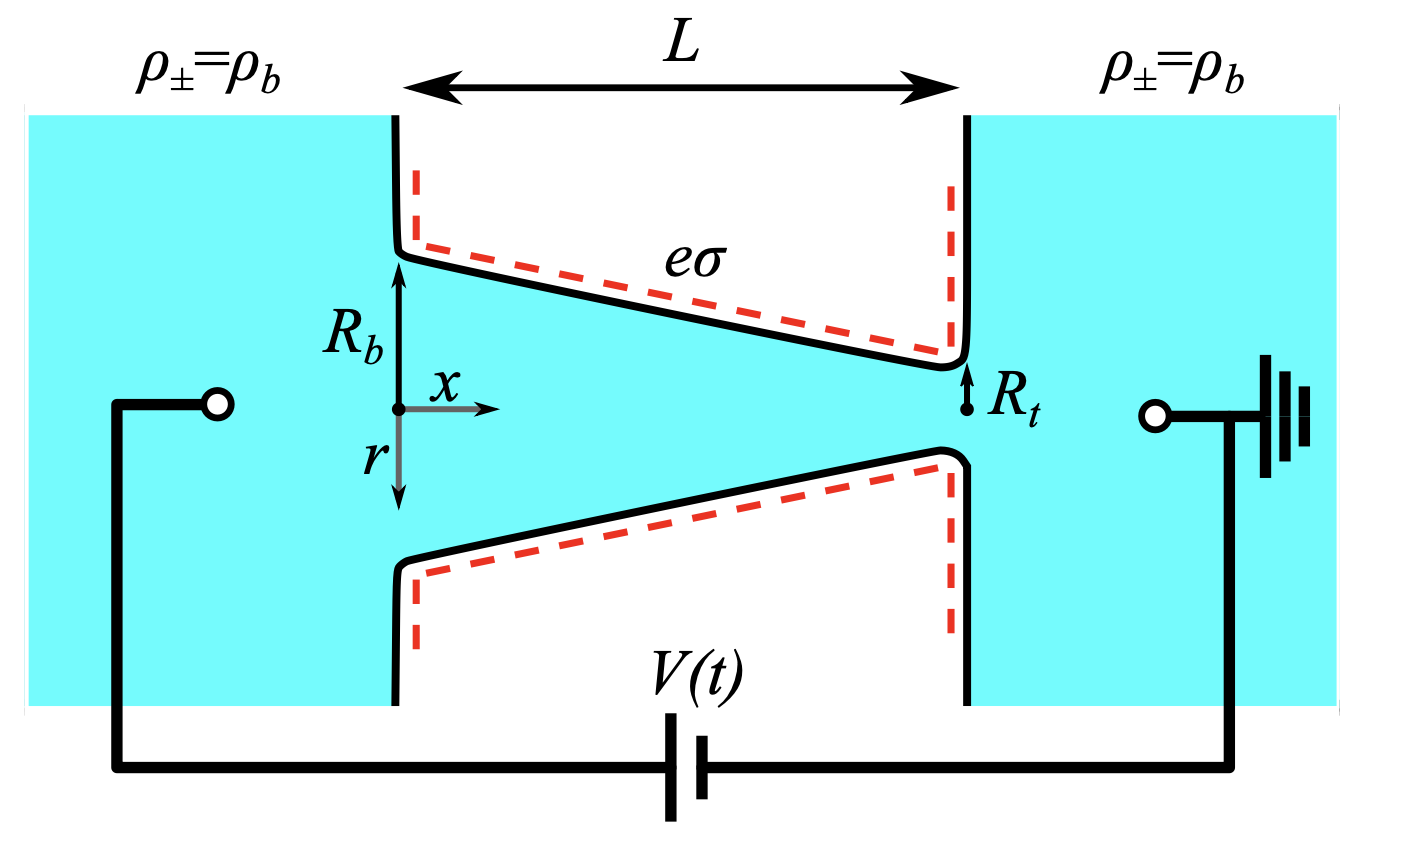
\includegraphics[width=0.5\columnwidth]{../figures_tex/conical_channel.png}
    \caption{Schematic representation of the conical channel we consider \cite{cone1}.}
    \label{fig:conical_channel}
\end{figure}

Transport in the channel is described by the PNPS equations, which were solved for this system in the stationary state version, i.e. with a static external potential $V$ \cite{cone3}. This results in a static charge current
\[
I = g_{\infty}(V)V
\]
where the static conductivity $g_{\infty}(V)$ was found to be governed by the voltage dependent radially averaged salt concentration $\bar{\rho}_s(x,V)$, here the salt concentration is $\rho_s = \rho_{+} + \rho_{-}$.

For small values of potential $V$, the average salt concentration in the cone equals the concentration in the bulk $\bar{\rho}_s(x,V)=2\rho_b$ and the conductance equals the Ohmic conductance
\[
g_{0}=\frac{\pi R_{t}R_{b}}{L}\frac{2\rho_b e^2 D}{k_B T}
\]
where $k_B=1.38\times 10^{-23}\text{JK}^{-1}$ is the Boltzmann constant and $T=293.15$K the temperature. The resulting current follows $I = g_0 V$.
For large static potential drops, the cone shows diodic behaviour as a consequence of the ion concentration polarization. This means that the current can flow through the cone in only one direction, due to the fact that the ions either accumulate or deplete in the channel, depending on the sign of the potential. In this regime, the cone conductance is found by solving the following
\begin{equation}
\frac{g_{\infty}(V)}{g_0} = 1 + \Delta g \int_{0}^{L}\left[ \frac{x R_t}{L R(x)} - \frac{e^{\text{Pe}(V)\frac{x R_t^2}{L R_b R(x)}}-1}{ e^{\text{Pe}(V)\frac{R_t}{R_b}} - 1 } \right] dx/L
\label{eq:cone_static}
\end{equation}
where Pe is the Péclet number, for the parameters chosen here $\text{Pe}(V)/V = 16.5 V^{-1}$. We show in \cref{fig:cone_steady_state} the steady state solution for a triangular shaped potential. A positive (negative) potential induces ion deplition (accumulation), thus low (high) conductivity, \cref{fig:cone_steady_state}(a). This gives rise to current rectification, shown in \cref{fig:cone_steady_state}(b) through the relation $I(V) = g_{\infty}(V) V$.
\begin{figure}[h]
    \centering
    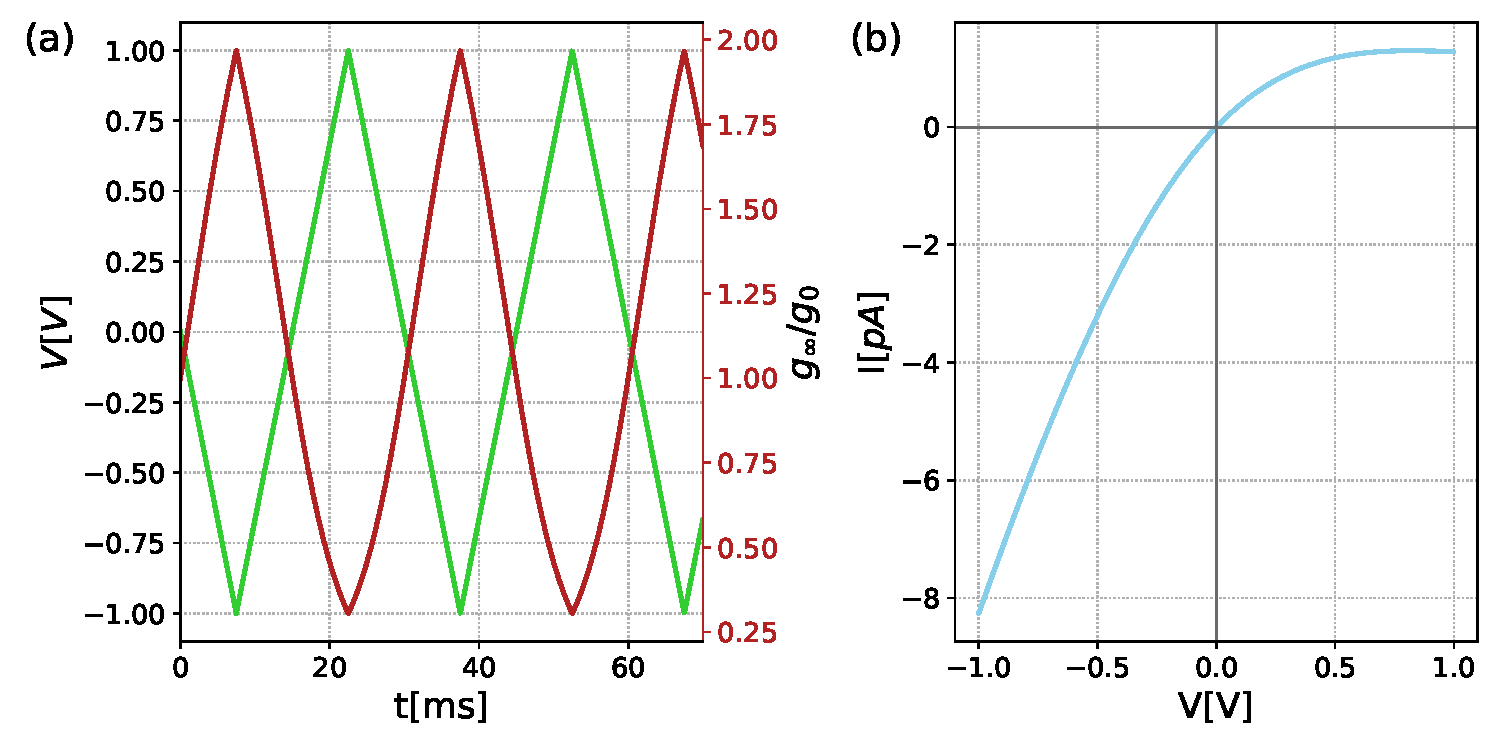
\includegraphics[width=0.7\columnwidth]{../figures_tex/cone_steady_state.pdf}
    \caption{(a) In green the shape of the potential and in red the stationary solution found by solving \cref{eq:cone_static}. In (b) the current found by $I(V) = g_{\infty}(V)V$.}
    \label{fig:cone_steady_state}
\end{figure}

It was shown that the process of accumulation and depletion occurs over a diffusion-like timescale \cite{tau_ref}. For the choice of parameters we made, this corresponds to $\tau = 4.8$ms.

We now decide to apply a time-dependent potential $V(t)$ and solve of the dynamics of the system. The time-dependent conductance $g(V(t),t)$ is analytically found by assuming an exponential relaxation of the salt concentration with timescale $\tau$ towards the steady-state, where the conductance is $g_{\infty}(V(t))$. This approach leads to the following differential equation for the conductance
\begin{equation}
\frac{\partial g(V(t),t)}{\partial t} = \frac{g_{\infty}(V(t))-g(V(t),t)}{\tau}
\label{eq:cone_dynam}
\end{equation}
which shows that the \textbf{conductance $g(V(t),t)$ depends on the entire timetrace of the potential.} The current is then found 
\[
I(V(t),t)=g(V(t),t)V(t).
\]
\begin{figure}[h]
    \centering
    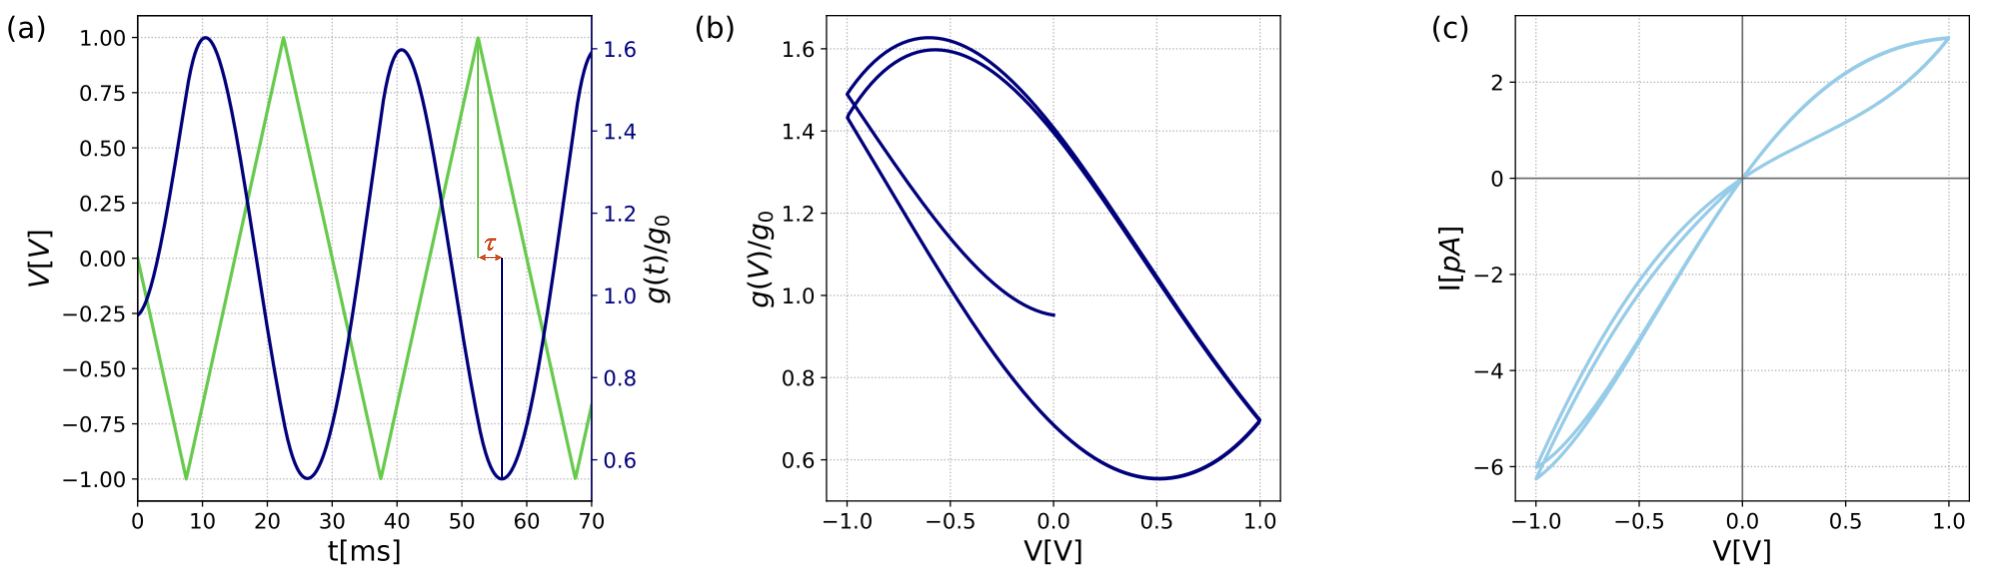
\includegraphics[width=1\columnwidth]{../figures_tex/cone_volt_cond_arrow.png}
    \caption{(a) In green the shape of the external potential applied and in blue the conductance of the cone in time. We show the relaxation time $\tau$ in red. (b) Conductance as a function of external potential. (c) Current as a function of external potential.}
    \label{fig:cone_steady_state}
\end{figure}
We show the result of the implementation in \cref{fig:cone_steady_state}. The hysteresis loop in both conductance and current is the hallmark of a memristor.

\newpage
\subsection{Simple Start: Voltage Divider}

The idea is now to apply the dynamics of memristors to the resistors in the network and find a smart potential that, applied at the edges of the resistors, would mimic the coupled learning training. Once again, we start with the simple voltage divider.

It is necessary to first adjust the system discussed in the previous sections in order to be able to compare its dynamics with the dynamics of memrisors at the same scales. In fact, we want to work with conductances instead of resistances and we want to scale their value from S to the order of $p$S. Also, we need to go from time-steps to real-time, associating a value of real-time to a single time-step. In \cref{fig:volt_con_mse_simp_cont} we show the training of conductances with continuous rule of \cref{eq:cond_update_cont} for the voltage divider. 
\begin{figure}[H]
    \centering
    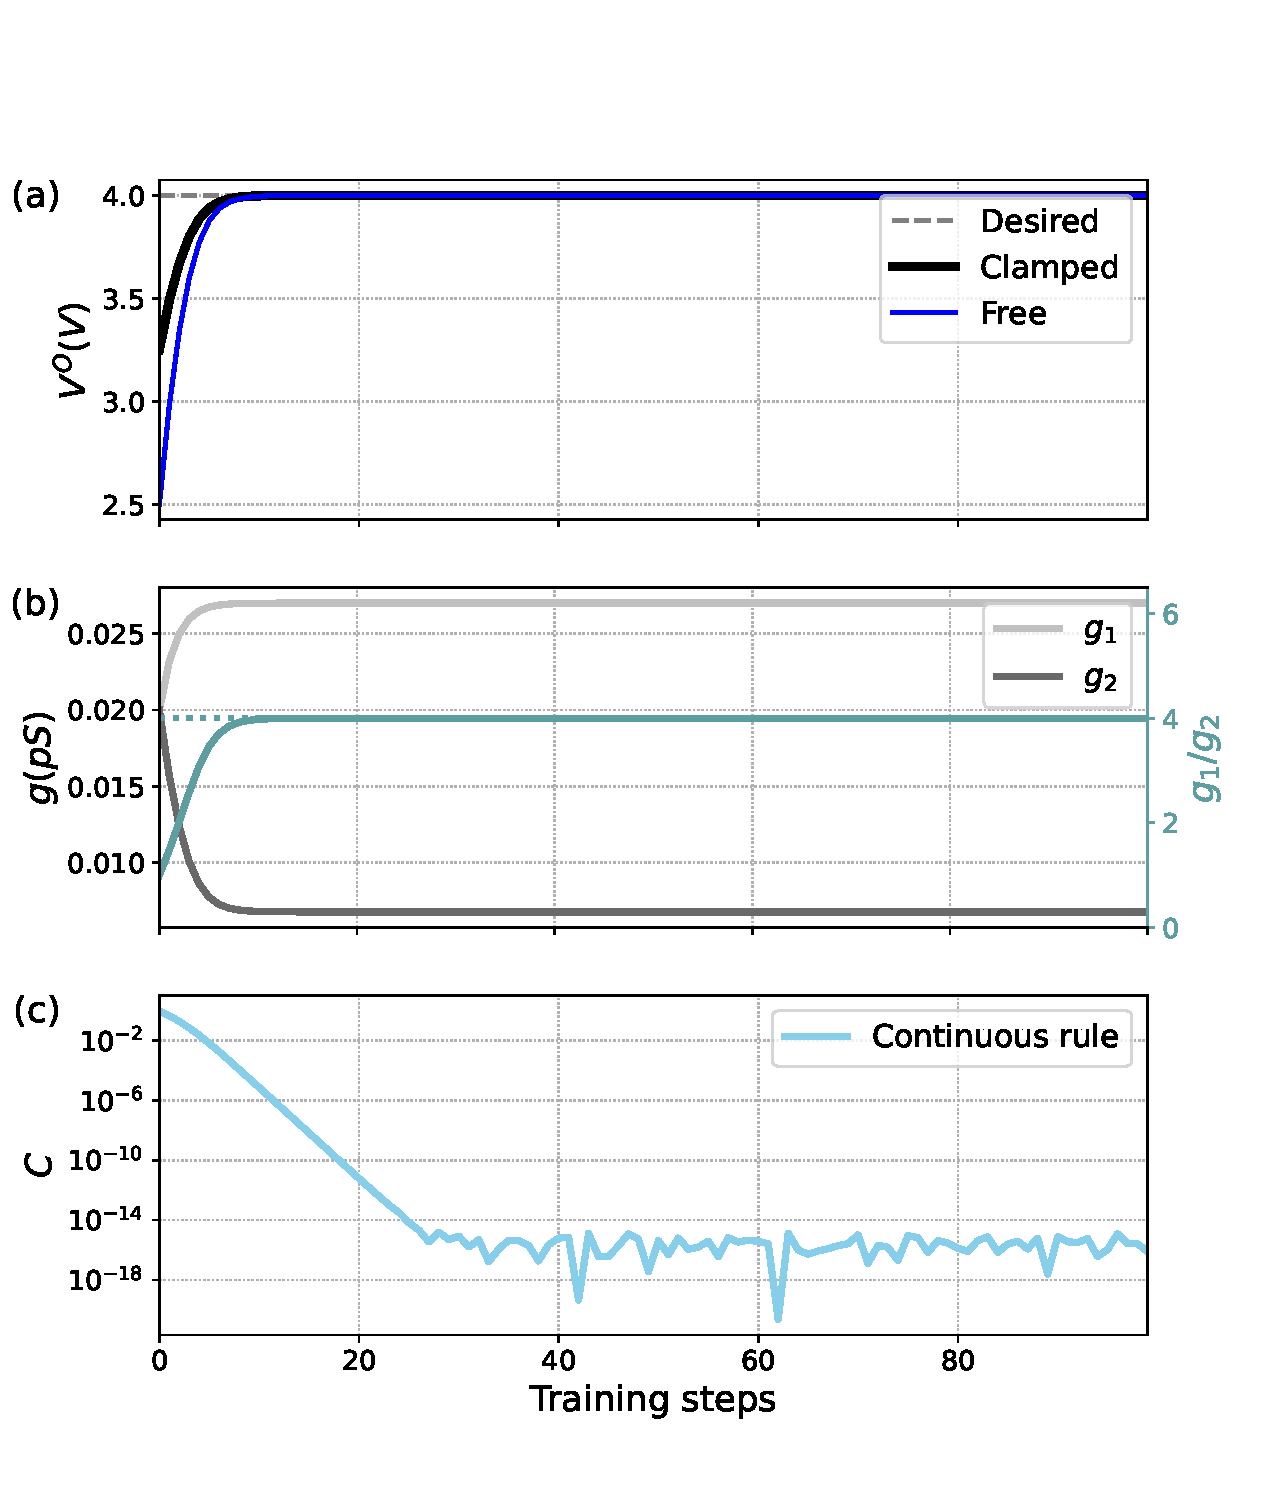
\includegraphics[width=0.5\columnwidth]{../figures_tex/volt_con_mse_simp_cont.pdf}
    \caption{Training a voltage divide within the coupled learning framework, but considering the conductances as learning degrees of freedom instead. Here we used $\eta=0.5$ and $\alpha=0.003$.}
    \label{fig:volt_con_mse_simp_cont}
\end{figure}
We started with an intial value for conductances of $1/50$S and adjusted the value of $\alpha$ in order to resemble the behaviour of the resistance, in \cref{fig:general_training_continuous}. Recall that the updating rule of the resistances, \cref{eq:cont_rul_res}, contains resistance squared in the denominator. Therefore, the magnitude and the value of the learning parameter $\gamma$ is different in the two cases, and the behaviour is not identical.


Before associating a real-time value to the training time-steps, we want to try changing the potential shape imposed at the edges of a conical channel, as illustrated in \cref{fig:cone_voltage}, and look at the behaviour of the conductance. 
\begin{figure}[h]
    \centering
    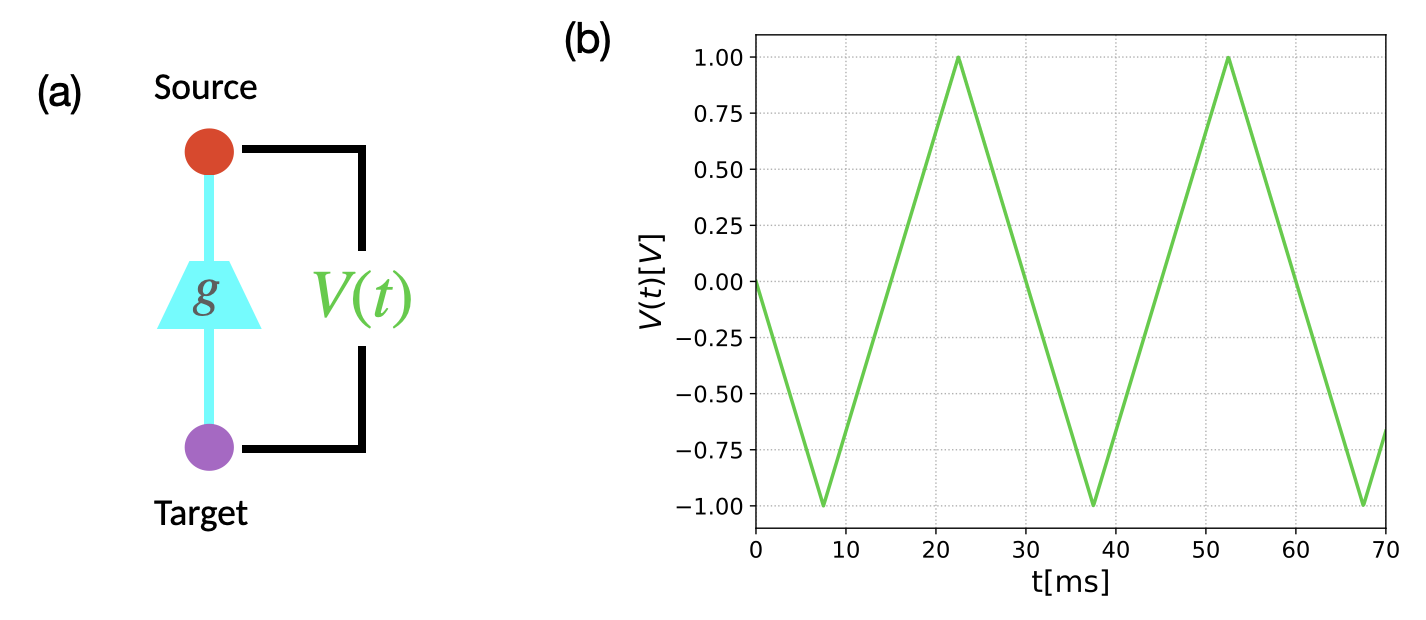
\includegraphics[width=0.6\columnwidth]{../figures_tex/cone_voltage.png}
    \caption{(a) The resistance has been substituted with a conical channel with conductance $g$. We play with the external potential applied, an example is showed in (b). }
    \label{fig:cone_voltage}
\end{figure}
In the end, we would like to obtain a behaviour similar to the one in \cref{fig:volt_con_mse_simp_cont}(b). 

Let us first consider the edge relative to the conductance $g_1$. It connects the source voltage, with $V_1 = 5V$, and the target voltage, in which we would like to have $V_D = 4V$. We first try to impose a potential shaped as a block function that, starting from $5V$ gives pulses to the desired potential of $4V$. We introduce the parameters used to model the square function, it has the equation
\[
V(t) = A  \ \text{signal.square}\left( 2\pi f \ t + \phi , \text{duty} \right) + V_{\text{shift}}
\]
where $A$ is the amplitude of the signal, $f$ the frequency, $\phi$ the phase and $V_{\text{shift}}$ a shift along the $y$-axis. This signal, in one period $T = 1/f$, assumes two values: $+V$ for $\delta t = T \cdot \text{duty}$ and $-V$, for $\Delta t = T - \delta t$. In \cref{fig:memtrain_volt_gsol} we show the behaviour of the conductance for this type of potential shape.
\begin{figure}[h]
    \centering
    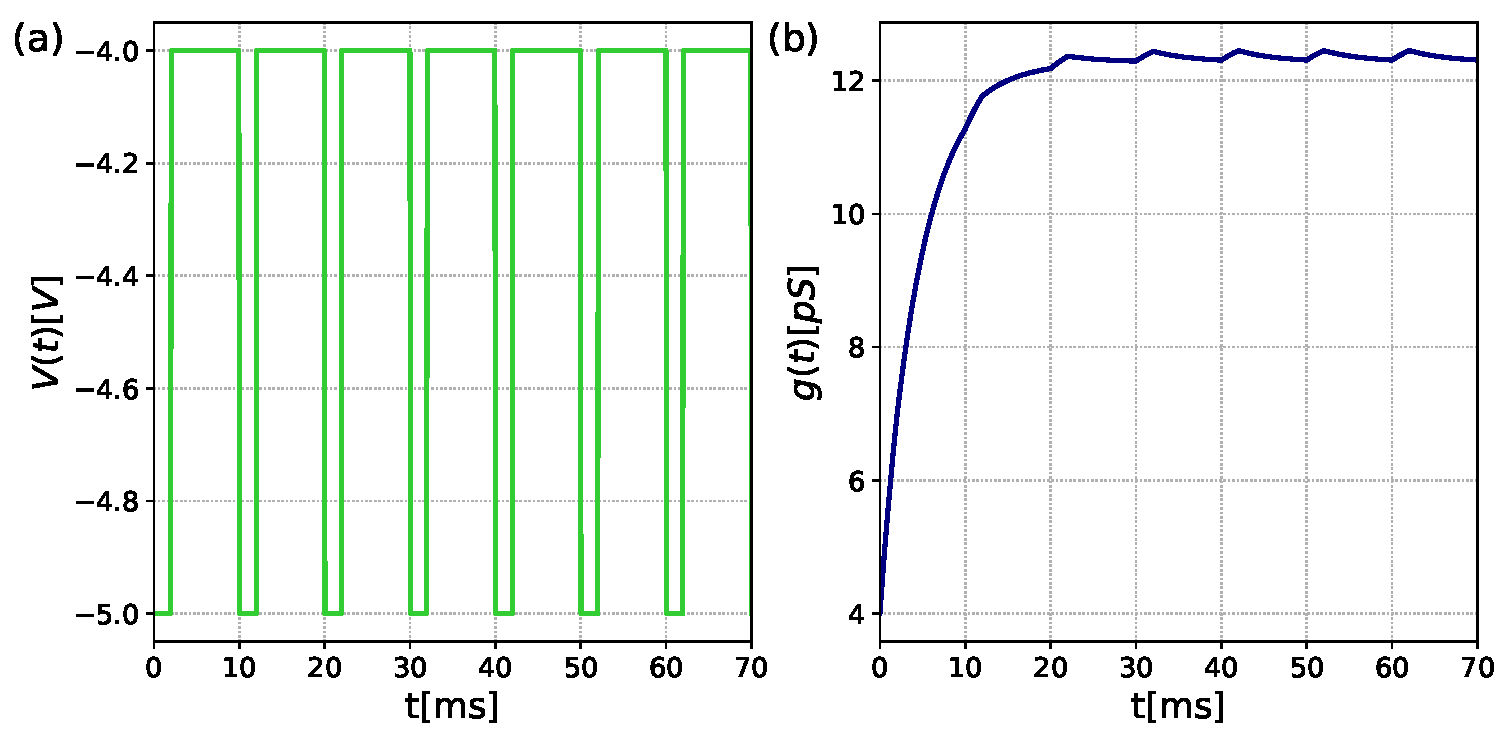
\includegraphics[width=0.7\columnwidth]{../figures_tex/memtrain_volt_gsol.pdf}
    \caption{(a) Potential shape: square wave with parameters $A=-1/2$, $f = 0.1$, $\phi=0$, duty$=0.2$ and $V_{\text{shift}}=-4.5$. With these parameters the pulses to the desired value of voltage $V_D=4$ last $\Delta t = 8$ms. (b) Conductance of the conical channel in time when external voltage in (a) is applied. The parameters have not changed, therefore $\tau = 4.8$ms.}
    \label{fig:memtrain_volt_gsol}
\end{figure}
In order for the conductance to grow, we need to impose a negative voltage. I observed that changing the initial condition $g(0)$ does not change the behaviour at longer times, the conductance always tends to the final value of approximately $12.3p$S. Changing $\Delta t$ only changes the length of the oscillations at longer times. 

With this, we build a voltage divider that has in one edge ($g_1$) a memristor and in the other ($g_2$) a resistor trained with coupled learning. The result in shown in \cref{fig:memr_coupled_simple}. We imposed the initial condition for the conductances to be $g(t=0)=4p$S, changing its value doesn't affect much the result. We perform $1000$ time-steps in both trainings. In order to have both trainings in real time, we associate a value of $0.07$ms to a training step in the coupled learning framework.
\begin{figure}[h]
    \centering
    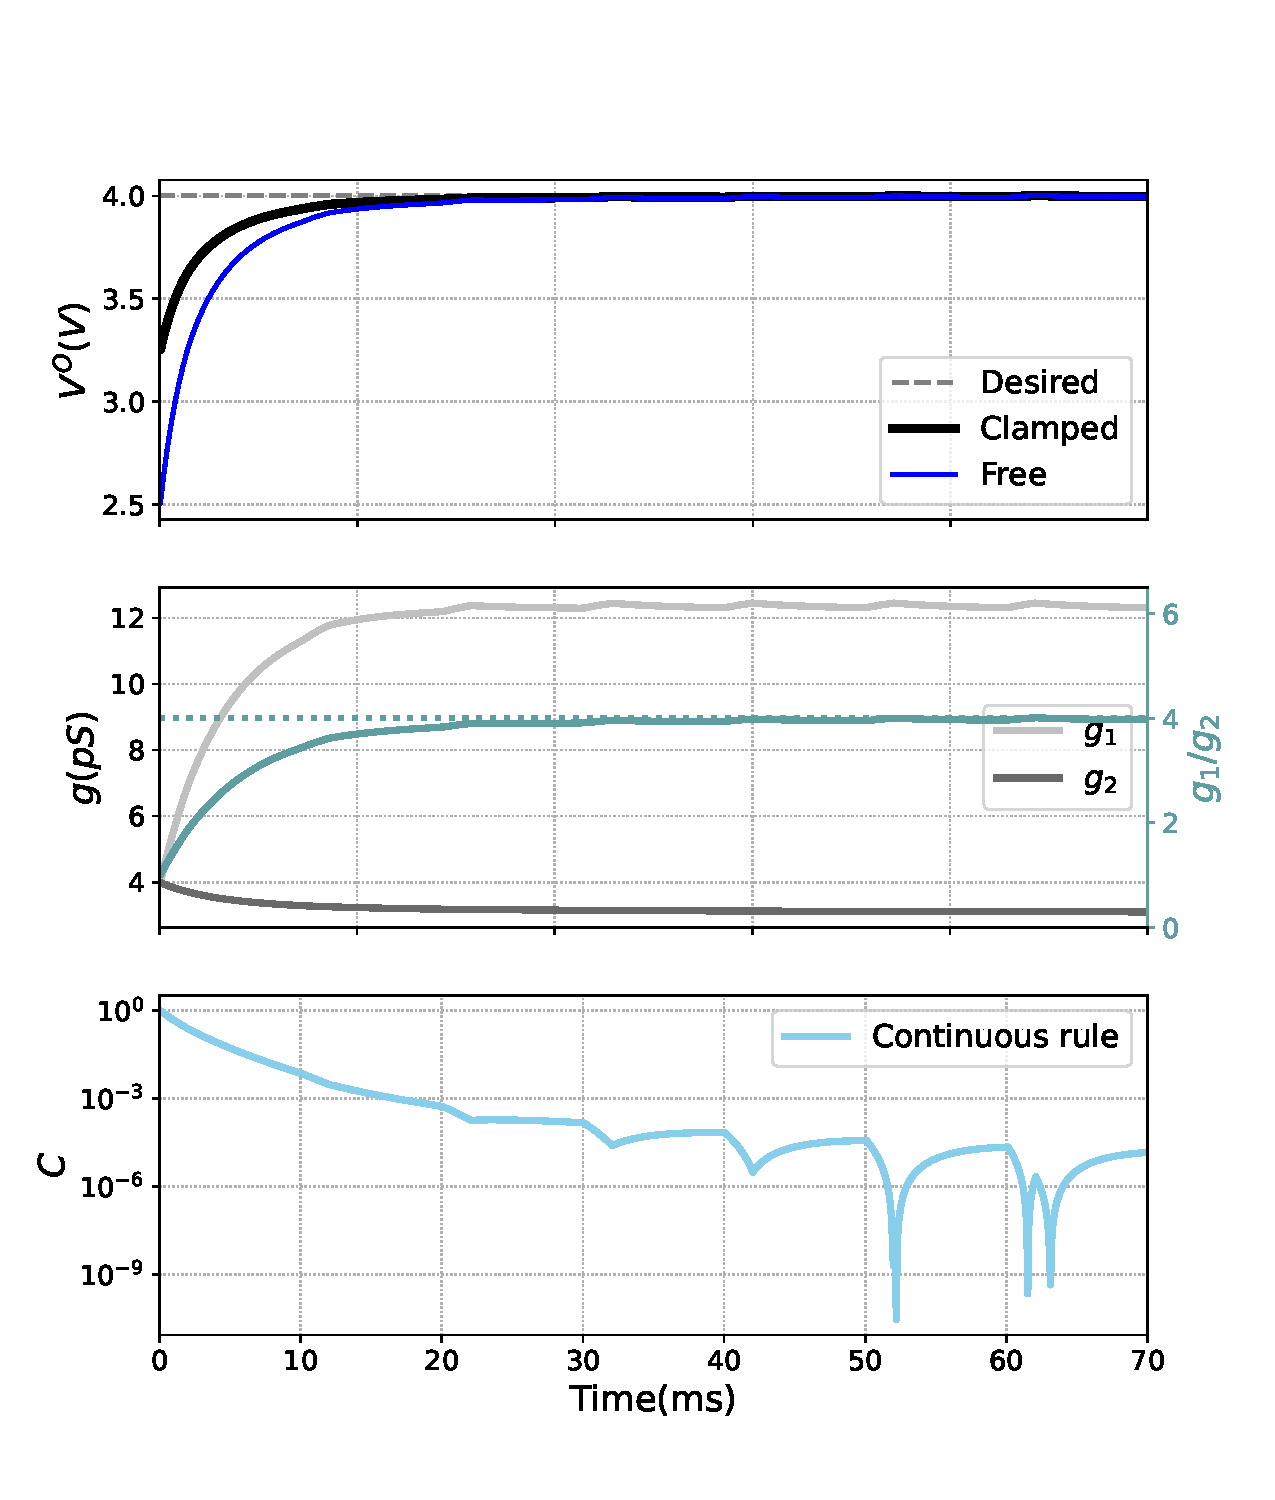
\includegraphics[width=0.6\columnwidth]{../figures_tex/memr_coupled_simple.pdf}
    \caption{Training the system with one memeristor ($g_1$) that follows the dynamics in \cref{eq:cone_dynam}, and a resistor ($g_2$) that follows coupled learning method.}
    \label{fig:memr_coupled_simple}
\end{figure}
It seems that the memristor follows its dynamic independently, while the resistor, with coupled learning, tries to adjust accordingly.

Regarding the memristor $g_2$, we apply another square wave potential, this time oscillating between the source potential $0V$ and the desired $4V$. In \cref{fig:memtrain_volt_gsol_g2} we show the result on the behaviour of the conductance.
\begin{figure}[h]
    \centering
    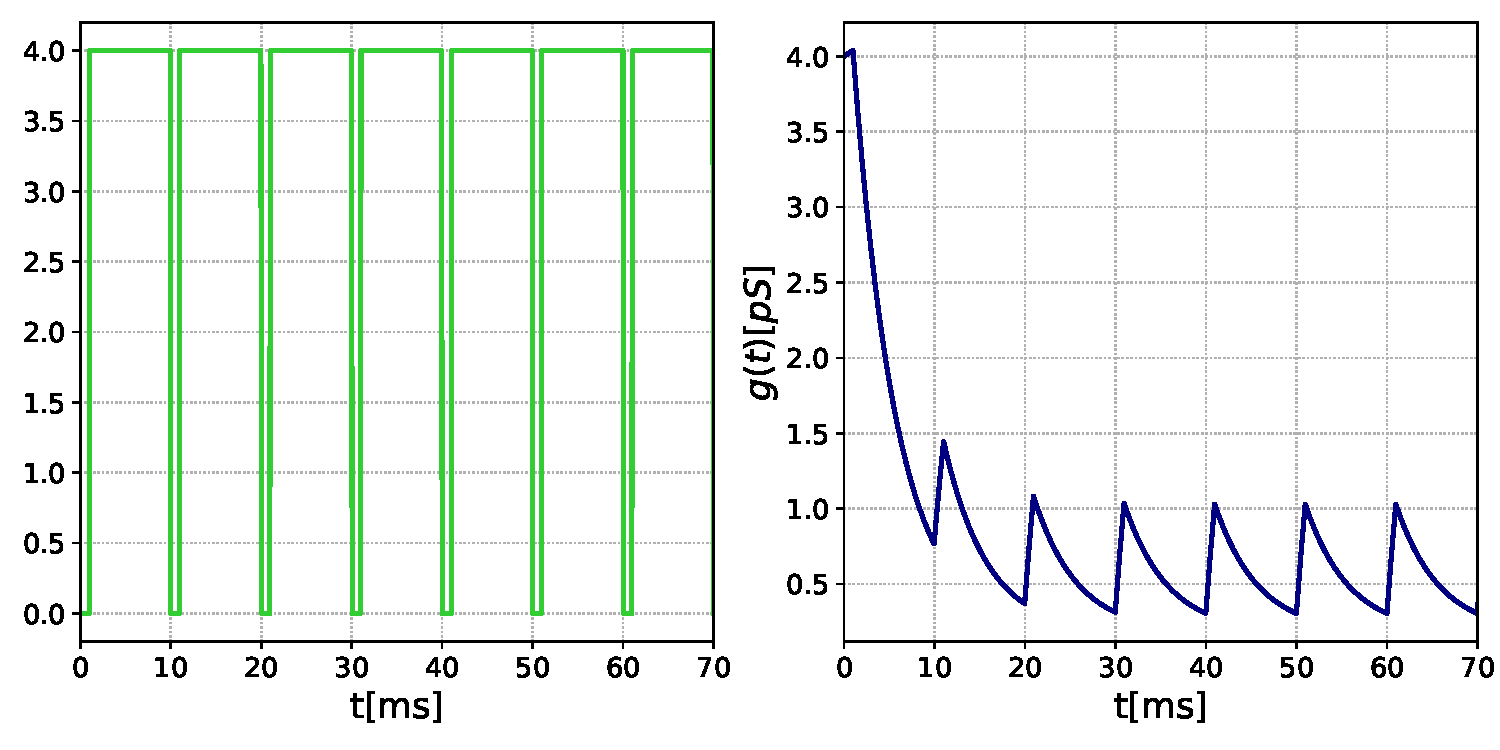
\includegraphics[width=0.7\columnwidth]{../figures_tex/memtrain_volt_gsol_g2.pdf}
    \caption{(a) Potential shape: square wave with parameters $A=-1/2$, $f = 0.1$, $\phi=0$, duty$=0.2$ and $V_{\text{shift}}=-4.5$. With these parameters the pulses to the desired value of voltage $V_D=4$ last $\Delta t = 8$ms. (b) Conductance of the conical channel in time when external voltage in (a) is applied. The parameters have not changed, therefore $\tau = 4.8$ms.}
    \label{fig:memtrain_volt_gsol_g2}
\end{figure}
Due to the larger difference between the values of the voltages with respect to the voltages in $g_1$, the oscillations at larger times are more marked.

We now try to substitute both the edges with memresistors. On $g_1$ we apply an external potential as in \cref{fig:memtrain_volt_gsol}, while on $g_2$ as in \cref{fig:memtrain_volt_gsol_g2}. The result is shown in \cref{fig:memr_memr_simple}.
\begin{figure}[h]
    \centering
    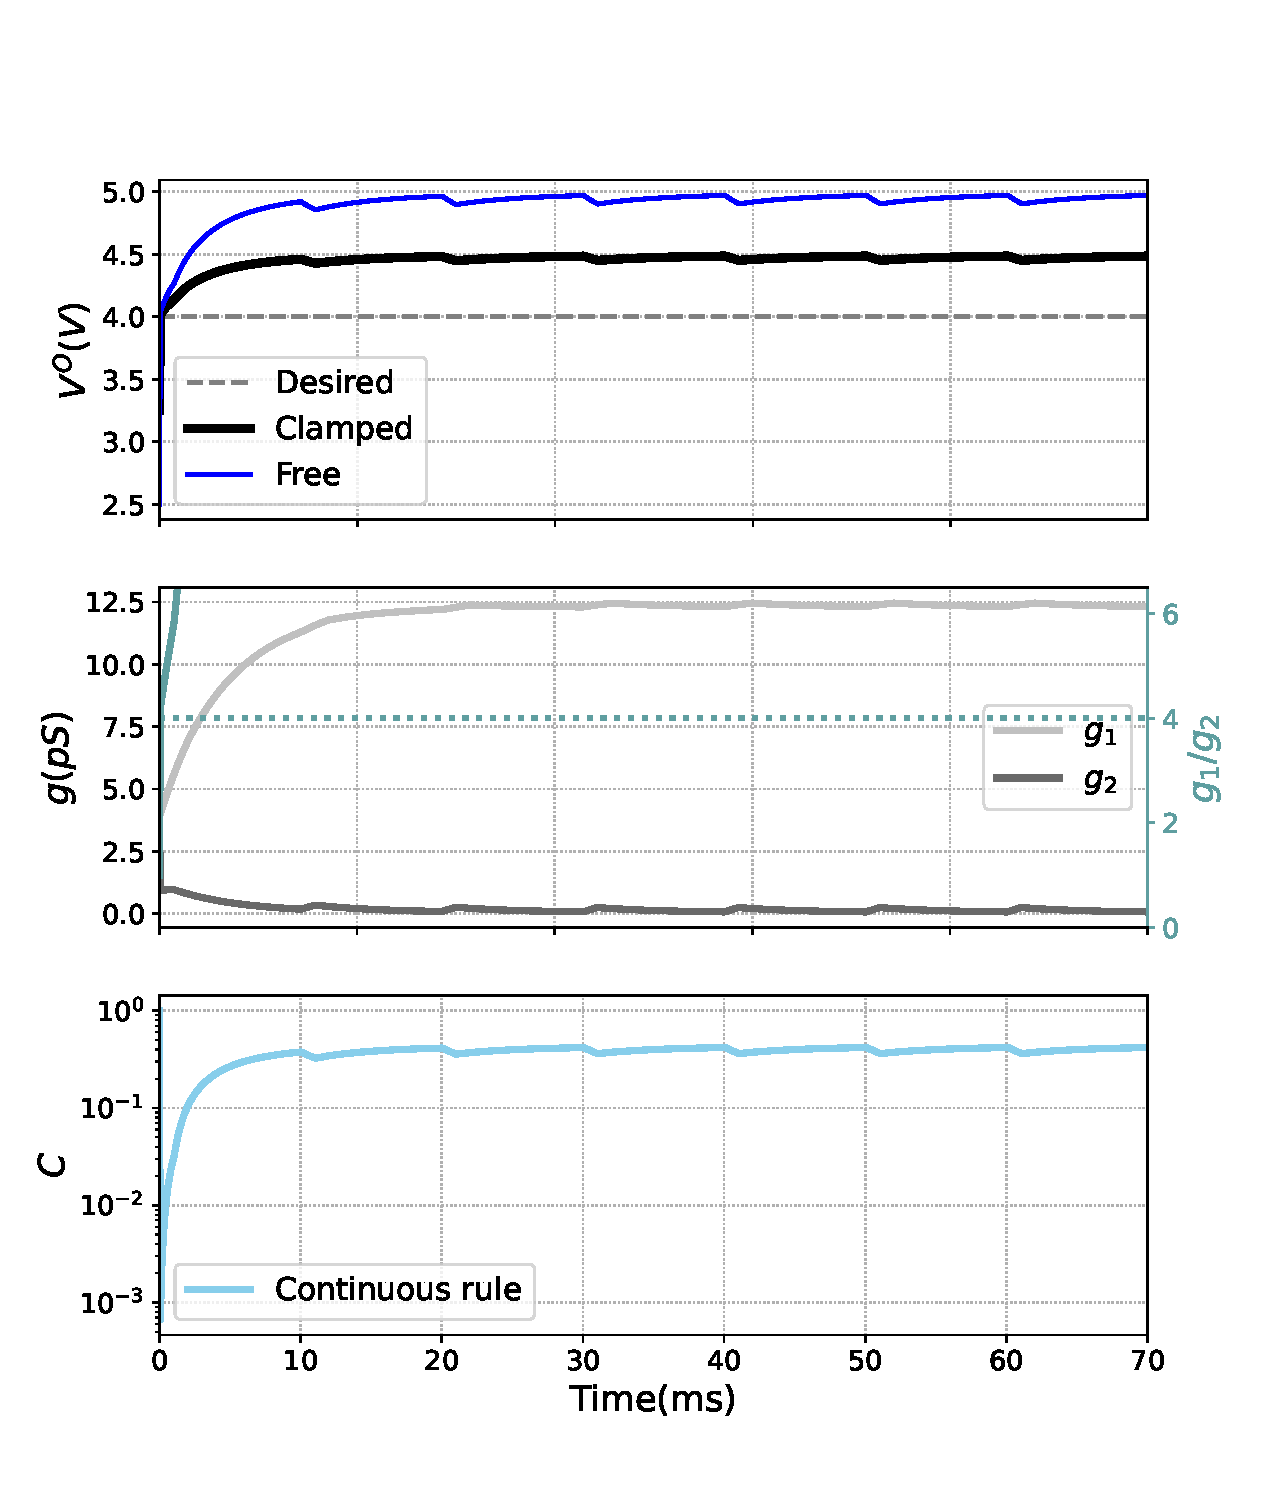
\includegraphics[width=0.6\columnwidth]{../figures_tex/memr_memr_simple.pdf}
    \caption{Training a voltage divider with two conical microfluidic channels connecting the nodes.}
    \label{fig:memr_memr_simple}
\end{figure}
The network this way does not get trained. This is plausable, the updating this way is independent of the state of the system and we are not using the memory properties of the memristor.  

With this machinery now working, we want to find a smart way of utilizing the memristors, at their full capacity.


\clearpage
%\printbibliography


\bibliographystyle{unsrt} 
\bibliography{biblio}

\end{document}

